\setcounter{section}{0}
\section{Lý thuyết}
\subsection{Cơ năng của một vật chuyển động trong trọng trường}
Khi một vật chuyển động trong trọng trường thì tổng động năng và thế năng của vật được gọi là cơ năng của vật trong trọng trường (gọi tắt là cơ năng của vật).

Kí hiệu cơ năng của vật là $W$:
\begin{equation*}
	W=W_\text{đ}+W_\text{t}=\dfrac{1}{2}mv^2+mgz\label{CT-conang},
\end{equation*}
trong đó:
\begin{itemize}
	\item $W$ là cơ năng của vật;
	\item $W_\text{đ}=\dfrac{1}{2}mv^2$ là động năng của vật;
	\item $W_\text{t}=mgz$ là thế năng của vật.
\end{itemize}

\subsection{Bảo toàn cơ năng của vật chuyển động trong trọng trường}
Khi một vật chuyển động trong trọng trường chỉ chịu tác dụng của trọng lực thì cơ năng của vật là một đại lượng bảo toàn.
\begin{equation*}
	W=W_\text{đ}+W_\text{t}=\dfrac{1}{2}mv^2+mgz=\textrm{hằng số}
\end{equation*}

\textit{Hệ quả:}
\begin{itemize}
	\item Nếu động năng giảm thì thế năng tăng (động năng chuyển hóa thành thế năng) và ngược lại.
	\item Tại vị trí nào động năng cực đại thì thế năng cực tiểu và ngược lại.
\end{itemize}
\ppgiai{
	\begin{description}
		\item[Bước 1:] Chọn mốc thế năng. Viết biểu thức cơ năng cho vị trí lúc đầu và lúc sau.
		
		Cơ năng cho vị trí lúc đầu, ta gọi là vị trí 1:
		\begin{equation*}
			W_1=W_\text{đ1}+W_\text{t1}=\dfrac{1}{2}mv_1^2+mgz_1.
		\end{equation*}
		
		Cơ năng cho vị trí lúc sau, ta gọi là vị trí 2:
		\begin{equation*}
			W_2=W_\text{đ2}+W_\text{t2}=\dfrac{1}{2}mv_2^2+mgz_2.
		\end{equation*}
		
		\item[Bước 2:] Áp dụng định luật bảo toàn cơ năng
		\begin{eqnarray*}
			W_1&=&W_2\\
			\Rightarrow W_\text{đ1}+W_\text{t1} &=& W_\text{đ2}+W_\text{t2}\\
			\Rightarrow \dfrac{1}{2}mv_1^2+mgz_1 &=& \dfrac{1}{2}mv_2^2+mgz_2.
		\end{eqnarray*}
	\end{description}
}
\subsection{Biến thiên cơ năng của vật chuyển động trong trọng trường}
Khi một vật chuyển động trong trọng trường, nếu vật chịu tác dụng thêm lực cản (không phải lực thế) thì cơ năng của vật sẽ biến đổi. Công của lực cản bằng độ biến thiên của cơ năng.
\begin{equation*}
	A=W_2-W_1,
\end{equation*}
trong đó:
\begin{itemize}
	\item $A$ là công của lực cản;
	\item $W_1$ là cơ năng lúc đầu ở vị trí 1;
	\item $W_2$ là cơ năng lúc sau ở vị trí 2.
\end{itemize}

\ppgiai{
	\begin{description}
		\item[Bước 1:] Chọn mốc thế năng. Viết biểu thức cơ năng cho vị trí lúc đầu và lúc sau.
		
		Cơ năng cho vị trí lúc đầu, ta gọi là vị trí 1:
		\begin{equation*}
			W_1=W_\text{đ1}+W_\text{t1}=\dfrac{1}{2}mv_1^2+mgz_1.
		\end{equation*}
		
		Cơ năng cho vị trí lúc sau, ta gọi là vị trí 2:
		\begin{equation*}
			W_2=W_\text{đ2}+W_\text{t2}=\dfrac{1}{2}mv_2^2+mgz_2.
		\end{equation*}
		
		\item[Bước 2:] Viết biểu thức tính công của lực cản (không phải lực thế) bằng độ biến thiên của cơ năng.
		\begin{equation*}
			A=W_2-W_1=\left(\dfrac{1}{2}mv_2^2+mgz_2\right)-\left(\dfrac{1}{2}mv_1^2+mgz_1\right).
		\end{equation*}
	\end{description}
}
\subsection{Biến thiên cơ năng của vật chịu tác dụng đồng thời của lực đàn hồi và lực không thế (đọc thêm)}
Khi vật chỉ chịu tác dụng của lực đàn hồi (là lực thế) thì cơ năng được bảo toàn. Nếu ngoài lực đàn hồi, vật chịu thêm tác dụng của một lực khác không phải là lực thế thì cơ năng không còn bảo toàn. Độ biến thiên cơ năng đúng bằng công của lực không thế:
\begin{equation*}
	A=W_2-W_1,
\end{equation*}
trong đó:
\begin{itemize}
	\item $A$ là công của lực không thế;
	\item $W_1$ là cơ năng lúc đầu ở vị trí 1;
	\item $W_2$ là cơ năng lúc sau ở vị trí 2.
\end{itemize}
\luuy{
	\begin{description}
		\item[Lực thế] là lực mà công sinh ra khi dịch chuyển vật chỉ phụ thuộc vị trí đầu và vị trí cuối của vật. Ví dụ: trọng lực, lực đàn hồi, lực tĩnh điện, $\ldots$;
		\item[Lực không thế] là lực mà công sinh ra khi dịch chuyển vật phụ thuộc vào đường đi của vật. Ví dụ: lực ma sát, lực cản không khí, $\ldots$.
	\end{description}
}
\ppgiai{
	\begin{description}
		\item[Bước 1:] Chọn mốc thế năng. Viết biểu thức cơ năng cho vị trí lúc đầu và lúc sau.
		
		Cơ năng cho vị trí lúc đầu, ta gọi là vị trí 1:
		\begin{equation*}
			W_1=W_\text{đ1}+W_\text{t1}=\dfrac{1}{2}mv_1^2+\dfrac{1}{2}k(\Delta l_1)^2.
		\end{equation*}
		
		Cơ năng cho vị trí lúc sau, ta gọi là vị trí 2:
		\begin{equation*}
			W_2=W_\text{đ2}+W_\text{t2}=\dfrac{1}{2}mv_2^2+\dfrac{1}{2}k(\Delta l_2)^2.
		\end{equation*}
		
		\item[Bước 2:] Viết biểu thức tính công của lực cản (không phải lực thế) bằng độ biến thiên của cơ năng.
		\begin{equation*}
			A=W_2-W_1=\left(\dfrac{1}{2}mv_2^2+\dfrac{1}{2}k(\Delta l_2)^2\right)-\left(\dfrac{1}{2}mv_1^2+\dfrac{1}{2}k(\Delta l_1)^2\right).
		\end{equation*}
	\end{description}
}
\section{Mục tiêu bài học - Ví dụ minh họa}
\begin{dang}{Biện luận sự chuyển hóa giữa động năng và thế năng}
	
	\viduii{2}{
		Một vật có khối lượng $m=\SI{1}{kg}$ được thả rơi tự do từ độ cao $\SI{20}{m}$ so với mặt đất. Chọn gốc thế năng tại mặt đất. Bỏ qua mọi ma sát. Ngay khi vật chạm đất thì
		\begin{mcq}
			\item động năng cực đại, thế năng cực tiểu.
			\item động năng bằng thế năng.
			\item động năng cực tiểu, thế năng cực đại.
			\item động năng bằng một nửa thế năng.
		\end{mcq}
	}
	{\begin{center}
			\textbf{Hướng dẫn giải}
		\end{center}
		
		Trong quá trình rơi, vận tốc của vật tăng dần còn độ cao giảm dần. Do đó, khi vật chạm đất thì vận tốc lớn nhất nên động năng cực đại, còn độ cao nhỏ nhất nên thế năng cực tiểu.
		
		\textbf{Đáp án: A}.
		
	}
	\viduii{2}{
		Một vật có khối lượng $m=\SI{1}{kg}$ được ném lên với vận tốc $\SI{10}{m/s}$ từ độ cao $\SI{1}{m}$ so với mặt đất. Chọn gốc thế năng tại mặt đất. Bỏ qua mọi ma sát. Ngay khi vật lên đến độ cao cực đại thì
		\begin{mcq}
			\item động năng cực đại, thế năng cực tiểu.
			\item động năng bằng thế năng.
			\item động năng cực tiểu, thế năng cực đại.
			\item động năng bằng một nửa thế năng.
		\end{mcq}
	}
	{\begin{center}
			\textbf{Hướng dẫn giải}
		\end{center}
		
		Trong quá trình vật bay lên, vận tốc giảm dần còn độ cao tăng dần. Do đó, khi vật lên đến độ cao cực đại thì thế năng cực đại vì độ cao cực đại, còn động năng cực tiểu vì vận tốc cực tiểu.
		
		\textbf{Đáp án: C}.
	}
\end{dang}
\begin{dang}{Xác định cơ năng của vật chuyển động trong trọng trường}
	\viduii{2}{Một vật có khối lượng $\SI{2}{kg}$ rơi tự do không vận tốc đầu từ độ cao $\SI{5}{m}$ xuống mặt đất. Nếu chọn gốc thế năng tại mặt đất, lấy $g=\SI{10}{m/s^2}$, cơ năng của vật có giá trị 
		\begin{mcq}(4)
			\item $\SI{10}{J}$.
			\item $\SI{100}{J}$.
			\item $\SI{50}{J}$.
			\item $\SI{5}{J}$.
		\end{mcq}
	}
	{	\begin{center}
			\textbf{Hướng dẫn giải}
		\end{center}
		Cơ năng của vật bằng tổng động năng và thế năng. Tại thời điểm bắt đầu rơi, vận tốc của vật bằng không, giá trị cơ năng tương ứng là 
		\begin{align*}
			W&=W_\text{đ}+W_\text{t}\\
			&=\dfrac{1}{2}mv^2+mgh\\
			&=\dfrac{1}{2}\cdot\SI{2}{\kilogram}\cdot(\SI{0}{\meter/\second})^2+\SI{2}{\kilogram}\cdot\SI{10}{\meter/\second^2}\cdot\SI{5}{\meter}\\
			&=\SI{100}{\joule}.
		\end{align*}
		
		\textbf{Đáp án: B.}
		
		\begin{center}
			\textbf{Câu hỏi tương tự}
		\end{center}
		
		Từ điểm M (có độ cao so với mặt đất bằng $\SI{0,8}{\meter}$) ném lên một vật với vận tốc đầu $\SI{2}{\meter/\second}$. Biết khối lượng của vật bằng $\SI{0,5}{\kilogram}$, lấy $g=\SI{10}{\meter/\second^2}$. Chọn mốc thế năng tại mặt đất, cơ năng của vật bằng bao nhiêu?
		
		\textbf{Đáp án:} $\SI{5}{\joule}$.
	}
	\viduii{3}{Một vật có khối lượng $\SI{100}{\gram}$ được ném thẳng đứng từ độ cao $\SI{5}{\meter}$ lên phía trên với vận tốc đầu là $\SI{10}{\meter/\second}$. Bỏ qua lực cản của không khí. Lấy $g=\SI{10}{\meter/\second^2}$. Xác định cơ năng của vật ở thời điểm $\SI{0,5}{\second}$ kể từ khi chuyển động.
	}
	{	\begin{center}
			\textbf{Hướng dẫn giải}
		\end{center}
		
		Chọn mặt đất là mốc thế năng, chiều dương là chiều từ mặt đất lên cao. Trường hợp này vật chuyển động chậm dần đều từ độ cao $z_0=\SI{5}{\meter}$ với gia tốc $g=\SI{-10}{\meter/\second^2}$ và vận tốc đầu $v_0=\SI{10}{\meter/\second}$.
		
		Vận tốc của vật đạt được sau thời $\SI{0,5}{\second}$ là
		\begin{equation*}
			v=v_0+gt=\SI{10}{\meter/\second}-\SI{10}{\meter/\second^2}\cdot\SI{0,5}{\second}=\SI{5}{\meter/\second}.
		\end{equation*}
		
		Độ cao của vật đạt được ở thời điểm $\SI{0,5}{\second}$ kể từ khi chuyển động là
		\begin{equation*}
			z=z_0+v_0t+\dfrac{1}{2}gt^2=\SI{5}{\meter}+\SI{10}{\meter/\second}\cdot\SI{0,5}{\second}-\dfrac{1}{2}\cdot\SI{10}{\meter/\second^2}\cdot(\SI{0,5}{\second})^2=\SI{8,75}{\meter}.
		\end{equation*}
		
		Cơ năng của vật ở thời điểm $\SI{0,5}{\second}$ kể từ khi chuyển động là
		\begin{equation*}
			W=\dfrac{1}{2}mv^2+mgz=\dfrac{1}{2}\cdot\SI{0,1}{\kilogram}\cdot(\SI{5}{\meter/\second})^2+\SI{0,1}{\kilogram}\cdot\SI{10}{\meter/\second^2}\cdot\SI{8,75}{\meter}=\SI{10}{\joule}.
		\end{equation*}
		
		Vậy cơ năng của vật ở thời điểm $\SI{0,5}{\second}$ kể từ khi chuyển động $\SI{10}{\joule}$.
		
		\textbf{\textit{Cách khác}} 
		
		Với lưu ý rằng vật chuyển động trong trọng trường và bỏ qua lực cản thì cơ năng của hệ được bảo toàn. Do đó cơ năng của vật ở thời điểm \SI{0.5}{\second} cũng bằng với cơ năng ở thời điểm ban đầu, và có giá trị 
		\begin{align*}
			W=\dfrac{1}{2}mv_0^2+mgz_0=\dfrac{1}{2}\cdot\SI{0.1}{\kilogram}\cdot(\SI{10}{\meter/\second})^2+\SI{0.1}{\kilogram}\cdot\SI{10}{\meter/\second^2}\cdot\SI{5}{\meter}=\SI{10}{\joule}.
		\end{align*}
		
		\begin{center}
			\textbf{Câu hỏi tương tự}
		\end{center}
		
		Một vật có khối lượng $\SI{100}{\gram}$ được ném thẳng đứng từ độ cao $\SI{3}{\meter}$ lên phía trên với vận tốc đầu là $\SI{15}{\meter/\second}$. Bỏ qua lực cản của không khí. Lấy $g=\SI{10}{\meter/\second^2}$. Xác định cơ năng của vật ở thời điểm $\SI{1}{\second}$ kể từ khi chuyển động.
		
		\textbf{Đáp án:} $\SI{14.25}{\joule}$.
	}
\end{dang}


\begin{dang}{Áp dụng định luật bảo toàn cơ năng cho vật rơi tự do }
	\viduii{2}{Một vật được ném theo phương thẳng đứng hướng xuống từ độ cao $\SI{15}{m}$ so với mặt đất với tốc độ $\SI{10}{m/s}$. Bỏ qua mọi lực cản. Chọn gốc thế năng tại mặt đất. Lấy $g=\SI{10}{m/s^2}$. Tốc độ của vật khi vật vừa chạm đất là
		\begin{mcq}(4)
			\item $\SI{10}{m/s}$.
			\item $\SI{15}{m/s}$.
			\item $\SI{20}{m/s}$.
			\item $\SI{400}{m/s}$.
		\end{mcq}
	}
	{	\begin{center}
			\textbf{Hướng dẫn giải}
		\end{center}
		
		Cơ năng của vật ở thời điểm đầu (khi vừa ném)
		\begin{align*}
			W_1=\dfrac{1}{2}mv_0^2+mgz_0
		\end{align*}
		Cơ năng của vật ở thời điểm cuối (khi chạm đất $z=0$)
		\begin{align*}
			W_2=\dfrac{1}{2}mv^2+mgz=\dfrac{1}{2}mv^2
		\end{align*}
		Bảo toàn cơ năng lúc vừa ném và lúc vừa chạm đất:
		\begin{align*}
			W_1&=W_2\\
			\Rightarrow\quad	\dfrac{1}{2}mv_0^2+mgz_0&=\dfrac{1}{2}mv^2\\
			\Rightarrow\quad v&=\sqrt{v_0^2+2gz_0}\\
			&=\sqrt{(\SI{10}{\meter/\second})^2+2\cdot\SI{10}{\meter/\second^2}\cdot\SI{15}{\meter}}\\
			&=\SI{20}{\meter/\second}.
		\end{align*}
		
		\textbf{Đáp án: C.}
		
		\begin{center}
			\textbf{Câu hỏi tương tự}
		\end{center}
		
		Một vật khối lượng $\SI{2}{kg}$ được ném thẳng đứng với vận tốc ban đầu $\SI{20}{m/s}$ xuống đất. Lấy $g=\SI{10}{m/s^2}$. Chọn gốc thế năng tại mặt đất. Bỏ qua lực cản của không khí trong quá trình vật chuyển động.
		\begin{enumerate}[label=\alph*)]
			\item Tính cơ năng của vật lúc ném.
			\item Tìm vận tốc của vật khi chạm đất.
		\end{enumerate}
		
		\textbf{Đáp án:} $\SI{400}{J}$; $\SI{20}{m/s}$.
	}
	\viduii{2}{Một vật được thả rơi tự do từ độ cao $\SI{3}{\meter}$. Xác định độ cao vật khi động năng bằng hai lần thế năng.
	}
	{	\begin{center}
			\textbf{Hướng dẫn giải}
		\end{center}
		
		Chọn mốc thế năng tại mặt đất.
		
		Tại vị trí thả, vật không có vận tốc nên động năng bằng không, cơ năng đúng bằng thế năng
		\begin{equation*}
			W_1=W_\text{đ1}+W_\text{t1}=0+W_\text{t1}=mgz_1.
		\end{equation*}
		
		Cơ năng của vật khi động năng bằng hai lần thế năng:
		\begin{equation*}
			W_2=W_\text{đ2}+W_\text{t2}=2W_\text{t2}+W_\text{t2}=3W_\text{t2}=3mgz_2.
		\end{equation*}
		
		Áp dụng định luật bảo toàn cơ năng
		\begin{eqnarray*}
			W_1&=&W_2\\
			\Rightarrow\quad mgz_1 &=& 3mgz_2\\
			\Rightarrow\quad z_1 &=& 3z_2\\
			\Rightarrow\quad z_2 &=& \dfrac{1}{3}z_1\\
			\Rightarrow\quad z_2 &=&\dfrac{1}{3}\cdot \SI{3}{\meter}=\SI{1}{\meter}.
		\end{eqnarray*}
		
		\begin{center}
			\textbf{Câu hỏi tương tự}
		\end{center}
		
		Vật có khối lượng $m=\SI{2}{kg}$ được thả rơi tự do từ độ cao $\SI{40}{m}$ so với mặt đất. Cho $g=\SI{10}{m/s^2}$. Chọn gốc thế năng tại mặt đất.
		\begin{enumerate}[label=\alph*)]
			\item Tính động năng của vật lúc chạm đất.
			\item Ở độ cao nào vật có động năng bằng thế năng?
		\end{enumerate}
		
		\textbf{Đáp án:} $\SI{800}{J}$; $\SI{20}{m}$.
	}
	\viduii{3}{
		Một vật ném thẳng đứng xuống dưới đất từ độ cao $\SI{5}{\meter}$. Khi chạm đất vật nảy trở lên với độ cao $\SI{7}{\meter}$. Bỏ qua mất mát năng lượng khi va chạm và sức cản môi trường. Lấy $g=\SI{10}{\meter/\second^2}$. Vận tốc ném ban đầu có giá trị bằng bao nhiêu?
	}
	{\begin{center}
			\textbf{Hướng dẫn giải}
		\end{center}
		
		Chọn mốc thế năng tại mặt đất.
		
		Cơ năng của vật tại vị trí thả là
		\begin{equation*}
			W_1=W_\text{đ1}+W_\text{t1}=\dfrac{1}{2}mv_1^2+mgz_1.
		\end{equation*}
		
		Cơ năng của vật tại vị trí vật nảy trở lên với độ cao $\SI{7}{\meter}$ là
		\begin{equation*}
			W_2=W_\text{đ2}+W_\text{t2}=W_\text{t2}=mgz_2.
		\end{equation*}
		
		Áp dụng định luật bảo toàn cơ năng
		\begin{eqnarray*}
			W_1&=&W_2\\
			\Rightarrow \dfrac{1}{2}mv_1^2+mgz_1 &=& mgz_2\\
			\Rightarrow \dfrac{1}{2}v_1^2+gz_1 &=& gz_2\\
			\Rightarrow v_1 &=& \sqrt{2g(h_2-h_1)}\\
			\Rightarrow v_1 &=& \sqrt{2\cdot\SI{10}{\meter/\second^2}\cdot(\SI{7}{\meter}-\SI{5}{\meter})}\\
			\Rightarrow v_1 &=& 2\sqrt{10}\,\text{m/s}.
		\end{eqnarray*}
		
		\begin{center}
			\textbf{Câu hỏi tương tự}
		\end{center}
		
		Một vật có khối lượng $\SI{2}{kg}$ được thả rơi tự do từ độ cao $\SI{2.5}{m}$ so với mặt đất. Lấy $g=\SI{10}{m/s^2}$, bỏ qua mọi lực cản của không khí. Chọn gốc thế năng ở mặt đất. Xác định vận tốc của vật khi đạt đến vị trí có độ cao giảm đi một nửa.
		
		\textbf{Đáp án: } $\SI{5}{m/s}$.
	}
\end{dang}

\begin{dang}{Áp dụng định luật bảo toàn cơ năng cho con lắc đơn}
	
	\viduii{3}{
		Một con lắc đơn gồm sợi dây nhẹ không dãn, chiều dài $\SI{50}{cm}$, một đầu cố định, đầu còn lại treo vật nặng có khối lượng $\SI{100}{g}$. Ban đầu vật nặng đứng yên ở vị trí cân bằng. Tại vị trí này, truyền cho vật nặng vận tốc $v_0=\SI{5}{m/s}$ theo phương ngang. Chọn gốc thế năng tại vị trí cân bằng và cho $g=\SI{10}{m/s^2}$.
		\begin{enumerate}[label=\alph*)]
			\item Tìm cơ năng của vật.
			\item Khi vật lên đến vị trí M có dây treo hợp với phương thẳng đứng góc $\alpha_\text M$, vật có thế năng bằng $1/4$ động năng. Hãy tính $\alpha_\text M$ và vận tốc của vật tại M.
		\end{enumerate}
	}
	{\begin{center}
			\textbf{Hướng dẫn giải}
		\end{center}
		
		\begin{enumerate}[label=\alph*)]
			\item 			
			Cơ năng của vật bằng tổng động năng và thế năng:
			$$W_1 = \dfrac{1}{2}mv_1^2 + mgz_1 = \dfrac{1}{2}mv_1^2 + 0 = \SI{1.25}{J}.$$
			
			\item Trong quá trình chuyển động, vật chịu tác dụng của trọng lực là lực thế, và lực căng dây luôn vuông góc với quỹ đạo là lực không sinh công. 
			Do đó cơ năng của vật đươc bảo toàn. 
			
			Khi thế năng bằng $1/4$ động năng thì động năng gấp 4 lần thế năng, cơ năng khi đó có thể tính theo công thức 
			\begin{align*}
				W_2 = W_\text{đ2} + W_\text{t2} = 4 W_\text{t2} + W_\text{t2} = 5 W_\text{t2} 
			\end{align*}
			Áp dụng định luật bảo toàn cơ năng, ta tính được độ cao của điểm M	
			\begin{align*}
				W_2= W_1 \quad\Rightarrow\quad 5mgz_2 = \dfrac{1}{2}mv_1^2 \quad \Rightarrow \quad z_2 = \dfrac{1}{10}\dfrac{v_1^2}{g}=\SI{0.25}{m}.
			\end{align*}
			Góc $\alpha_\text M$ giữa phương thẳng đứng và phương dây treo được tính theo công thức: $\cos \alpha_\text M = \dfrac{l-z_2}{l} = \dfrac{1}{2}$, suy ra $\alpha_\text M = 60^\circ$.
			
			Vận tốc của vật tại M:
			$$W_\text{đ2} = 4 W_\text{t2} \Rightarrow \dfrac{1}{2}mv_2^2 = 4 mgz_2 \Rightarrow v_2 = \xsi{2\sqrt 5}{m/s}.$$
		\end{enumerate}
		
	}
	\viduii{3}{
		Một dây nhẹ dài $l=\SI{1}{m}$ đầu trên cố định, đầu dưới treo một vật nặng khối lượng $m$. Người ta kéo cho dây treo lệch một góc $\alpha = 60^\circ$ so với phương thẳng đứng rồi thả nhẹ cho vật chuyển động. Lấy $g=\SI{10}{m/s^2}$. Bỏ qua lực cản của không khí.
		\begin{enumerate}[label=\alph*)]
			\item Xác định vận tốc vật khi vật đi qua vị trí mà dây treo hợp với phương thẳng đứng một góc $\beta = 30^\circ$.
			\item Chứng minh rằng tại vị trí dây treo thẳng đứng vận tốc của vật có độ lớn cực đại, tìm giá trị cực đại đó.
		\end{enumerate}
	}
	{\begin{center}
			\textbf{Hướng dẫn giải}
		\end{center}
		
		\begin{enumerate}[label=\alph*)]
			\item Xác định vận tốc vật khi vật đi qua vị trí mà dây treo hợp với phương thẳng đứng một góc $\beta = 30^\circ$.
			
			Chọn gốc thế năng tại vị trí cân bằng của vật. Áp dụng định luật bảo toàn cơ năng:
			$$W_1 = W_2 \Rightarrow mgl(1-\cos \alpha) + 0 = \dfrac{1}{2} mv_2^2 + mgl (1-\cos \beta) \Rightarrow v_2 = \SI{2.7}{m/s}.$$
			
			\item Chứng minh rằng tại vị trí dây treo thẳng đứng vận tốc của vật có độ lớn cực đại, tìm giá trị cực đại đó.
			
			Tại vị trí dây treo thẳng đứng thì thế năng $z_3=0$, do đó động năng cực đại, dẫn đến vận tốc cực đại.
			
			Áp dụng bảo toàn cơ năng:
			$$W_1 = W_3 \Rightarrow mgl(1-\cos \alpha) = \dfrac{1}{2}mv_3^2 \Rightarrow v_3 = \xsi{\sqrt{10}}{m/s}.$$
		\end{enumerate}
		
		\begin{center}
			\textbf{Câu hỏi tương tự}
		\end{center}
		
		Một con lắc đơn có sợi dây dài $\SI{1}{\meter}$ và vật nặng có khối lượng $\SI{500}{\gram}$. Kéo vật lệch khỏi vị trí cân bằng sao cho cho dây làm với đường thẳng đứng một góc $60^\circ$ rồi thả nhẹ. Lấy $g= \SI{10}{\meter/\second^2}$.
		\begin{enumerate}[label=\alph*)]
			\item Xác định cơ năng của con lắc đơn trong quá trình chuyển động.
			\item Tính vận tốc của con lắc khi nó đi qua vị trí mà dây làm với đường thẳng đứng góc $30^\circ$, $45^\circ$ và xác định lực căng của dây ở hai vị trí đó. Lấy $g= \SI{10}{\meter/\second^2}$.
			\item Xác định vị trí để vật có vận tốc $v=\SI{1,8}{\meter/\second}$.
			\item Xác định vận tốc vật tại vị trí $2W_\text{t}=W_\text{đ}$.
			\item Xác định vị trí để $2W_\text{t}=3W_\text{đ}$. Tính vận tốc vật và lực căng dây khi đó.
		\end{enumerate}
		
		\textbf{Đáp án:} $\SI{2.5}{J}$; $\SI{2.7}{m/s}$; $\SI{2.0}{m/s}$; $48,54^\circ$; $\SI{2.58}{m/s}$; $\SI{2}{m/s}$; $\SI{5.5}{N}$.
	}
\end{dang}

\begin{dang}{Áp dụng biến thiên cơ năng để xác định quãng đường, vận tốc}
	\viduii{3}{Một vật có khối lượng $m=\SI{1}{\kilogram}$ rơi không vận tốc đầu từ độ cao $z_1$ so với mặt đất trong không khí,  lấy gia tốc trọng trường $g=\SI{10}{\meter/\second^2}$. Khi vật đi được $\SI{3}{\meter}$, biết lực cản trung bình của không khí ngược chiều với chuyển động và có độ lớn $\SI{4}{\newton}$, thì độ lớn vận tốc của vật là
		\begin{mcq}(4)
			\item $\SI{4,0}{\meter/\second}$.
			\item $\SI{7,7}{\meter/\second}$.
			\item $\SI{8,9}{\meter/\second}$.
			\item $\SI{6,0}{\meter/\second}$.
		\end{mcq}
	}
	{	\begin{center}
			\textbf{Hướng dẫn giải}
		\end{center}
		\begin{center}
			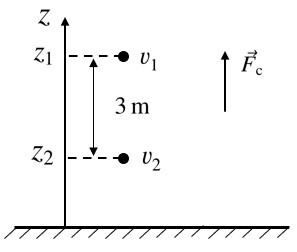
\includegraphics[scale=0.6]{../figs/VN10-PH-33-L-025-3-H1.jpg}
		\end{center}
		Công của lực cản khi vật chuyển động $\SI{3}{\meter}$ là
		\begin{equation*}
			A=F_\text{c}S\cos\alpha=\SI{4}{\newton}\cdot\SI{3}{\meter}\cdot\cos(180^\circ)=\SI{-12}{\joule}.
		\end{equation*}
		
		Cơ năng của vật lúc bắt đầu rơi là
		\begin{equation*}
			W_1=W_\text{đ1}+W_\text{t1}=\dfrac{1}{2}mv_1^2+mgz_1=mgz_1.
		\end{equation*}
		
		Cơ năng của vật sau khi rơi quãng đường $\SI{3}{\meter}$ là
		\begin{equation*}
			W_2=W_\text{đ2}+W_\text{t2}=\dfrac{1}{2}mv_2^2+mgz_2.
		\end{equation*}
		
		Do vật chịu tác dụng thêm lực cản nên cơ năng vật biến đổi. Công của lực cản bằng độ biến thiên cơ năng
		\begin{eqnarray*}
			A&=&W_2-W_1\\
			\Rightarrow A &=& \dfrac{1}{2}mv_2^2+mgz_2 - mgz_1\\
			\Rightarrow A &=& \dfrac{1}{2}mv_2^2+mg(z_2-z_1)\\
			\Rightarrow \SI{-12}{\joule} &=& \dfrac{1}{2}\cdot\SI{1}{\kilogram}\cdot v_2^2 + \cdot\SI{1}{\kilogram}\cdot \SI{10}{\meter/\second^2}\cdot(-\SI{3}{\meter})\\
			\Rightarrow v_2 &=& \SI{6}{\meter/\second}.
		\end{eqnarray*}
		
		\textbf{Đáp án: D.}
		
		\begin{center}
			\textbf{Câu hỏi tương tự}
		\end{center}
		
		Một vật khối lượng $\SI{2}{kg}$ được ném thẳng đứng với vận tốc ban đầu $\SI{20}{m/s}$ xuống đất. Lấy $g=\SI{10}{m/s^2}$. Chọn gốc thế năng tại mặt đất. Bỏ qua lực cản của không khí trong quá trình vật chuyển động.
		\begin{enumerate}[label=\alph*)]
			\item Tính cơ năng của vật lúc ném.
			\item Tìm vận tốc của vật khi chạm đất.
		\end{enumerate}
		
		\textbf{Đáp án:} $\SI{400}{J}$; $\SI{20}{m/s}$.
	}
	\viduii{3}{Một vật có khối lượng $m$ bắt đầu trượt không vận tốc đầu từ đỉnh của một mặt phẳng nghiêng có hệ số ma sát $\mu=0,2$, góc nghiêng $\beta=30^\circ$, $g=\SI{10}{\meter/\second^2}$. Khi vật trượt được quãng đường dài $\SI{10}{\meter}$ trên mặt phẳng nghiêng thì vận tốc của vật là
		\begin{mcq}(4)
			\item $\SI{8}{\meter/\second}$.
			\item $\SI{7}{\meter/\second}$.
			\item $\SI{9}{\meter/\second}$.
			\item $\SI{10}{\meter/\second}$.
		\end{mcq}
	}
	{	\begin{center}
			\textbf{Hướng dẫn giải}
		\end{center}
		
		\textbf{Cách 1:}
		
		\begin{center}
			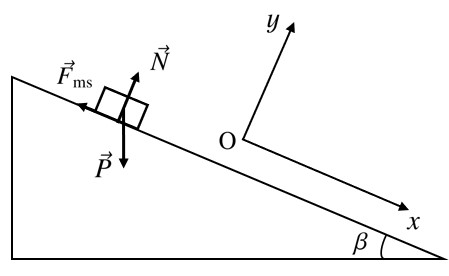
\includegraphics[scale=0.5]{../figs/VN10-PH-33-L-025-3-H2.jpg}
		\end{center}
		
		Chọn O$x$ và O$y$ như hình vẽ.
		
		Các lực tác dụng gồm:
		\begin{itemize}
			\item Lực ma sát $\vec{F}_\text{ms}$;
			\item Trọng lực $\vec{P}$;
			\item Phản lực $\vec{N}$.
		\end{itemize}
		
		Áp dụng định luật II Newton ta được
		\begin{equation*}
			\vec{a}=\dfrac{\vec{P}+\vec{N}+\vec{F}_\text{ms}}{m}.
		\end{equation*}
		
		Chiếu lên O$y$ ta được
		\begin{equation*}
			N = P\cos\beta = mg\cos\beta.
		\end{equation*}
		
		Chiếu lên O$x$ ta được
		\begin{equation*}
			a=\dfrac{P\sin\beta-F_\text{ms}}{m}=\dfrac{mg\sin\beta-\mu mg\cos\beta}{m}=g(\sin\beta-\mu\cos\beta).
		\end{equation*}
		
		Thay số vào ta được
		\begin{equation*}
			a=g(\sin\beta-\mu\cos\beta)=\SI{10}{\meter/\second^2}\cdot (\sin30^\circ-0,2\cdot\cos30^\circ)=\SI{3,27}{m/s^2}.
		\end{equation*}
		
		Theo công thức liên hệ a, v, s trong chuyển động thẳng biến đổi đều ta có
		\begin{equation*}
			v^2-v_0^2=2as\Rightarrow v=\sqrt{v_0^2+2as}=\sqrt{2\cdot (\SI{3,27}{m/s^2}\cdot \SI{10}{\meter}}= \SI{8}{\meter/\second}.
		\end{equation*}
		
		Vậy khi vật trượt được quãng đường dài $\SI{10}{\meter}$ trên mặt phẳng nghiêng thì vận tốc của vật là $\SI{8}{\meter/\second}$.
		
		\textbf{Cách 2:}
		
		\begin{center}
			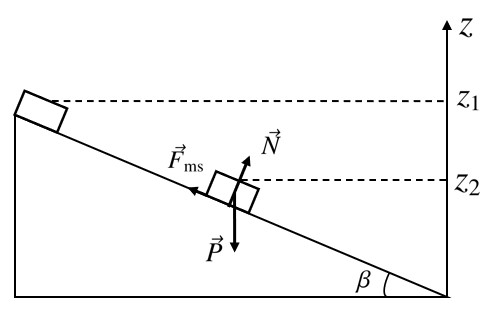
\includegraphics[scale=0.5]{../figs/VN10-PH-33-L-025-3-H3.jpg}
		\end{center}
		
		Chọn mốc thế năng tại vị trí chân mặt phẳng nghiêng.
		
		Các lực tác dụng gồm:
		\begin{itemize}
			\item Lực ma sát $\vec{F}_\text{ms}$;
			\item Trọng lực $\vec{P}$;
			\item Phản lực $\vec{N}$.
		\end{itemize}
		
		Công của lực không thế tác dụng lên vật là
		\begin{eqnarray*}
			A&=&A_\text{ms}+A_N\\
			&=&F_\text{ms}s\cos\alpha+0\\
			&=&\mu N s\cos\alpha\\
			&=&\mu\cdot  mg\cos\beta \cdot s \cdot \cos\alpha
		\end{eqnarray*}
		
		Cơ năng của vật lúc bắt đầu rơi là
		\begin{equation*}
			W_1=W_\text{đ1}+W_\text{t1}=\dfrac{1}{2}mv_1^2+mgz_1=mgz_1.
		\end{equation*}
		
		Cơ năng của vật sau khi rơi quãng đường $\SI{10}{\meter}$ là
		\begin{equation*}
			W_2=W_\text{đ2}+W_\text{t2}=\dfrac{1}{2}mv_2^2+mgz_2
		\end{equation*}
		
		Do vật chịu tác dụng thêm lực cản nên cơ năng vật biến đổi. Công của lực cản bằng độ biến thiên cơ năng
		\begin{eqnarray*}
			A&=&W_2-W_1\\
			\Rightarrow A &=& \dfrac{1}{2}mv_2^2+mgz_2 - mgz_1\\
			\Rightarrow \mu\cdot  mg\cos\beta \cdot s \cdot \cos\alpha &=& \dfrac{1}{2}mv_2^2+mg(z_2 - z_1)\\
			\Rightarrow \mu\cdot  g\cos\beta \cdot s \cdot \cos\alpha &=& \dfrac{1}{2}v_2^2 - g s\sin\beta\\
			\Rightarrow 0,2 \cdot \SI{10}{\meter/\second^2} \cdot \cos 30^\circ \cdot \SI{10}{\meter} \cdot \cos 180^\circ &=& \dfrac{1}{2}\cdot v_2^2 -\SI{10}{\meter/\second^2}\cdot \SI{10}{\meter} \cdot\sin30^\circ\\
			\Rightarrow v_2 &=& \SI{8}{\meter/\second}.
		\end{eqnarray*}
		
		\textbf{Đáp án: A}.
		
		\begin{center}
			\textbf{Câu hỏi tương tự}
		\end{center}
		
		Một viên bi khối lượng $m$ chuyến động ngang không ma sát với vận tốc $\SI{2}{\meter/\second}$ rồi đi lên mặt phẳng nghiêng góc nghiêng $30^\circ$.
		\begin{enumerate}[label=\alph*)]
			\item Tính quãng đường $s$ mà viên bi đi được trên mặt phẳng nghiêng.
			\item Ở độ cao nào thì vận tốc của viên bi giảm còn một nửa?
			\item Khi vật chuyển động được quãng đường là $\SI{0,2}{\meter}$ lên mặt phẳng nghiêng thì vật có vận tốc bao nhiêu?
		\end{enumerate}
		
		\textbf{Đáp án:} $\SI{0.4}{m}$; $\SI{0.15}{m}$; $\xsi{\sqrt 2}{m/s}$.
	}
	
\end{dang}

\begin{dang}{Áp dụng biến thiên cơ năng  để xác định lực tác dụng }
	
	\viduii{3}{
		Một vật khối lượng $\SI{2}{kg}$ được ném thẳng đứng với vận tốc ban đầu $\SI{20}{m/s}$ xuống đất. Lấy $g=\SI{10}{m/s^2}$. Chọn gốc thế năng tại mặt đất. Bỏ qua lực cản của không khí trong quá trình vật chuyển động. Sau khi chạm đất, vật lún sâu $\SI{10}{cm}$ rồi dừng lại. Tính lực cản trung bình của đất.
	}
	{\begin{center}
			\textbf{Hướng dẫn giải}
		\end{center}
		
		Cơ năng của vật tại ví trí ném:
		$$W_1 = W_\text{đ1} + W_\text{t1} = \SI{400}{J}.$$
		
		Cơ năng của vật tại vị trí sâu $\SI{10}{cm}$ dưới đất:
		$$W_2 = 0 + mgz_2 = \SI{-2}{J}.$$
		
		Khi vật dừng lại thì toàn bộ cơ năng chuyển thành công của lực cản của đất:
		$$\Delta W = W_2 - W_1 = \SI{-402}{J}= A_\text{cản} = -F_\text{cản} \cdot \SI{0.1}{m} \Rightarrow F_\text{cản} = \SI{4020}{N}.$$
		
		\begin{center}
			\textbf{Câu hỏi tương tự}
		\end{center}
		
		Một viên bi nhỏ khối lượng $\SI{200}{g}$ được ném thẳng đứng xuống dưới từ điểm O có độ cao $\SI{7}{m}$ so với mặt đất với tốc độ ban đầu $\SI{4}{m/s}$. Bỏ qua sức cản của không khí, lấy $g=\SI{10}{m/s^2}$. Giải bài toán bằng phương pháp năng lượng, chọn gốc thế năng tại mặt đất. Đất mềm, viên bi lún thẳng xuống mặt đất thêm một đoạn $\SI{10}{cm}$. Tính lực cản trung bình của đất tác dụng lên viên bi.
		
		\textbf{Đáp án:} $\SI{158}{N}$.
	}
	\viduii{3}{
		Ném vật khối lượng $\SI{150}{g}$ thẳng đứng lên cao từ mặt đất với vận tốc $\SI{20}{m/s}$. Cho $g=\SI{10}{m/s^2}$. Chọn gốc thế năng tại mặt đất.
		
		Nếu lực cản trung bình của không khí bằng $20\%$ trọng lượng của vật thì độ cao cực đại mà vật đạt được là bao nhiêu?
	}
	{\begin{center}
			\textbf{Hướng dẫn giải}
		\end{center}
		
		Cơ năng:
		$$W_1 = W_\text{đ1} + 0 =\dfrac{1}{2}mv_0^2=\dfrac{1}{2}\cdot\SI{0.15}{\kilogram}\cdot(\SI{20}{\meter/\second})^2= \SI{30}{J}.$$
		
		Lực cản bằng trung bình của không khí tác dụng lên vật  $$F_\text{cản} = 20\%mg = 20\%\cdot\SI{0.15}{\kilogram}\cdot\SI{10}{\meter/\second^2}= \SI{0.3}{\newton}.$$
		
		Công của lực cản tác dụng lên vật từ khi vật ở mặt đất đến khi vật ở độ cao cực đại $h$:
		$$A_\text{cản} = -F_\text{cản} h.$$
		
		Độ biến thiên cơ năng bằng công của lực cản:
		$$\Delta W = W_2 - W_1 = mgh - W_1 = -F_\text{cản} h \Rightarrow h= \SI{16.67}{m}.$$
		
		\begin{center}
			\textbf{Câu hỏi tương tự}
		\end{center}
		
		Một vật có khối lượng $\SI{3}{kg}$ được thả rơi không vận tốc đầu từ độ cao $\SI{4}{m}$ so với mặt đất. Lấy $g=\SI{9.8}{m/s^2}$. Biết ngay trước khi chạm đất vận tốc của vật là $\SI{6}{m/s}$. Hãy tính lực cản trung bình của không khí tác dụng lên vật.
		
		\textbf{Đáp án:} $\SI{15.9}{N}$.
	}
\end{dang}
\begin{dang}{Áp dụng biến thiên cơ năng của vật chịu tác dụng đồng thời \\của lực đàn hồi và lực không thế (đọc thêm)}
	\viduii{4}{Một con lắc lò xo gồm vật nhỏ khối lượng $\SI{2}{\kilogram}$ và lò xo có độ cứng $\SI{100}{\newton/\meter}$. Vật nhỏ được đặt trên giá đỡ cố định, nằm ngang dọc theo trục lò xo. Hệ số ma sát trượt giữa giá đỡ và vật nhỏ là $\mu=0,1$. Ban đầu giữ vật ở vị trí lò xo dãn $\Delta l_1=\SI{10}{\centi\meter}$ rồi buông nhẹ $v_1=0$. Lấy $g=\SI{10}{\meter/\second^2}$. Khi lò xo trở về trạng thái tự nhiên lần đầu tiên $\Delta l_2=0$ thì động năng của vật có giá trị bằng
		\begin{mcq}(4)
			\item $\SI{0,3}{\joule}$.
			\item $\SI{0,2}{\joule}$.
			\item $\SI{0,5}{\joule}$.
			\item $\SI{0,8}{\joule}$.
		\end{mcq}
	}
	{	\begin{center}
			\textbf{Hướng dẫn giải}
		\end{center}
		\begin{center}
			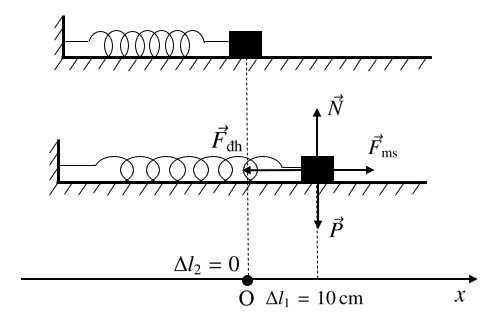
\includegraphics[scale=0.6]{../figs/VN10-PH-33-L-025-6-H1.jpg}
		\end{center}
		
		Các lực tác dụng gồm:
		\begin{itemize}
			\item Lực ma sát $\vec{F}_\text{ms}$;
			\item Trọng lực $\vec{P}$;
			\item Phản lực $\vec{N}$;
			\item Lực đàn hồi $\vec{F}_\text{đh}$.
		\end{itemize}
		
		Công của lực cản tác dụng lên vật là
		\begin{eqnarray*}
			A_\text{ms}&=&F_\text{ms}s\cos\alpha\\
			&=&\mu mg s \cos\alpha\\
			&=& 0,1\cdot\SI{2}{\kilogram}\cdot\SI{10}{\meter/\second^2}\cdot\SI{0,1}{\meter}\cdot\cos 180^\circ\\
			&=&\SI{-0,2}{\joule}.
		\end{eqnarray*}
		
		Cơ năng của vật lúc đầu (thời điểm buông vật) là
		\begin{equation*}
			W_1=W_\text{đ1}+W_\text{t1}=W_\text{t1}=\dfrac{1}{2}k(\Delta l_1)^2=\dfrac{1}{2}\cdot\SI{100}{\newton/\meter}\cdot(\SI{0,1}{\meter})^2=\SI{0,5}{\joule}.
		\end{equation*}
		
		Cơ năng của vật khi về đến vị trí tự nhiên của lò xo
		\begin{equation*}
			W_2=W_\text{đ2}+W_\text{t2}=W_\text{đ2}.
		\end{equation*}
		
		Do vật chịu tác dụng thêm lực ma sát nên cơ năng của vật sẽ biến đổi. Công của lực cản bằng độ biến thiên cơ năng. Từ đó ta tính được động năng của vật tại vị trí lần đầu tiên $\Delta l_2=0$ là
		\begin{eqnarray*}
			A_\text{ms}&=&W_2-W_1\\
			\Rightarrow \SI{-0,2}{\joule}&=&W_\text{đ2}-\SI{0,5}{\joule}\\
			\Rightarrow W_\text{đ2}&=&\SI{0,3}{\joule}.
		\end{eqnarray*}
		
		\textbf{Đáp án: A}.
	}
	\viduii{4}{
		Một con lắc lò xo gồm vật nhỏ khối lượng $\SI{1}{\kilogram}$ và lò xo có độ cứng $\SI{100}{\newton/\meter}$. Vật nhỏ được đặt trên giá đỡ cố định, nằm ngang dọc theo trục lò xo. Hệ số ma sát trượt giữa giá đỡ và vật nhỏ là $\mu=0,1$. Ban đầu giữ vật ở vị trí lò xo dãn $\Delta l_1=\SI{10}{\centi\meter}$ rồi buông nhẹ $v_1=0$. Lấy $g=\SI{10}{\meter/\second^2}$. Khi vật đi được quãng đường $s=\SI{8}{\centi\meter}$ thì vật có vận tốc bằng
		\begin{mcq}(4)
			\item $\SI{0,8}{\meter/\second}$.
			\item $\SI{0,9}{\meter/\second}$.
			\item $\SI{0,7}{\meter/\second}$.
			\item $\SI{0,6}{\meter/\second}$.
		\end{mcq}
	}
	{\begin{center}
			\textbf{Hướng dẫn giải}
		\end{center}
		
		\begin{center}
			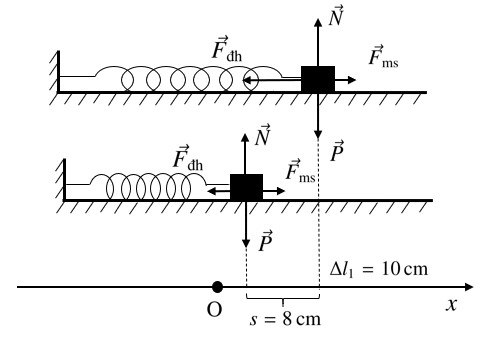
\includegraphics[scale=0.6]{../figs/VN10-PH-33-L-025-6-H2.jpg}
		\end{center}
		
		Các lực tác dụng gồm:
		\begin{itemize}
			\item Lực ma sát $\vec{F}_\text{ms}$;
			\item Trọng lực $\vec{P}$;
			\item Phản lực $\vec{N}$;
			\item Lực đàn hồi $\vec{F}_\text{đh}$.
		\end{itemize}
		
		Công của lực cản tác dụng lên vật là
		\begin{eqnarray*}
			A_\text{ms}&=&F_\text{ms}s\cos\alpha\\
			&=&\mu mg s \cos\alpha\\
			&=& 0,1\cdot\SI{1}{\kilogram}\cdot\SI{10}{\meter/\second^2}\cdot\SI{0,08}{\meter}\cdot\cos 180^\circ\\
			&=&\SI{-0,08}{\joule}.
		\end{eqnarray*}
		
		Cơ năng của vật lúc đầu (buông nhẹ) là
		\begin{equation*}
			W_1=W_\text{đ1}+W_\text{t1}=W_\text{t1}=\dfrac{1}{2}k(\Delta l_1)^2=\dfrac{1}{2}\cdot\SI{100}{\newton/\meter}\cdot(\SI{0,1}{\meter})^2=\SI{0,5}{\joule}.
		\end{equation*}
		
		Cơ năng của vật sau khi đi được quãng đường $\SI{8}{\centi\meter}$ là
		\begin{equation*}
			W_2=W_\text{đ2}+W_\text{t2}=\dfrac{1}{2}mv_2^2+\dfrac{1}{2}k(\Delta l_2)^2=\dfrac{1}{2}mv_2^2+\dfrac{1}{2}k(\Delta l_1 - s)^2.
		\end{equation*}
		
		Do vật chịu tác dụng thêm lực ma sát nên cơ năng của vật sẽ biến đổi. Công của lực cản bằng độ biến thiên cơ năng
		\begin{eqnarray*}
			A_\text{ms}&=&W_2-W_1\\
			\Rightarrow A_\text{ms}&=&\dfrac{1}{2}mv_2^2+\dfrac{1}{2}k(\Delta l_1 - S)^2-\SI{0,5}{\joule}\\
			\Rightarrow \SI{-0,08}{\joule}&=&\dfrac{1}{2}\cdot\SI{1}{\kilogram}\cdot v_2^2+\dfrac{1}{2}\cdot \SI{100}{\newton/\meter}\cdot (\SI{0,1}{\meter} - \SI{0,08}{\meter})^2-\SI{0,5}{\joule}.\\
			\Rightarrow \left|v_2\right|  &\approx& \SI{0,9}{\meter/\second}.
		\end{eqnarray*}
		
		Vậy khi vật đi được quãng đường $s=\SI{8}{\centi\meter}$ thì vật có vận tốc bằng $\SI{0,9}{\meter/\second}$.
		
		\textbf{Đáp án: B}.
	}
\end{dang}
\section{Tự luận}
\begin{enumerate}[label=\bfseries Câu \arabic*:]

	\item \mkstar{2}
	
	
	{
		Từ điểm A cách mặt đất $\SI{1}{m}$, một vật có khối lượng $\SI{0.5}{kg}$ được ném thẳng đứng lên trên với vận tốc $\SI{4}{m/s}$. Lấy $g=\SI{10}{m/s^2}$. Bỏ qua sức cản của không khí. Chọn gốc thế năng tại mặt đất. Tính cơ năng của vật tại vị trí ném.
	}
	
	\hideall
	{	
		Cơ năng của vật bằng tổng động năng và thế năng:
		$$W=mgz+\dfrac{1}{2}mv^2 = \SI{9}{J}.$$
	}
	\item \mkstar{2}
	
	
	{
		Người ta ném một quả bóng có khối lượng $m=\SI{200}{g}$ từ độ cao $\SI{2}{m}$ so với mặt đất lên cao với vận tốc $\SI{5}{m/s}$. Cho $g=\SI{10}{m/s^2}$. Chọn gốc thế năng tại mặt đất. Tính động năng, thế năng, cơ năng của quả bóng tại vị trí ném.
	}
	
	\hideall
	{	
		Động năng:
		$$W_\text{đ} = \dfrac{1}{2}mv^2 = \SI{2.5}{J}.$$
		
		Thế năng:
		$$W_\text t = mgz = \SI{4}{J}.$$
		
		Cơ năng:
		$$W=W_\text{đ} + W_\text t = \SI{6.5}{J}.$$
	}
	\item \mkstar{3}
	
	
	{
		Ném thẳng đứng xuống dưới một vật khối lượng $\SI{200}{g}$ với vận tốc $\SI{5}{m/s}$ từ độ cao $\SI{1.5}{m}$ so với mặt đất. Bỏ qua mọi lực cản. Cho $g=\SI{10}{m/s^2}$. Tính động năng, thế năng và cơ năng của vật
		\begin{enumerate}[label=\alph*)]
			\item ngay lúc ném.
			\item ngay trước khi chạm đất.
		\end{enumerate}
	}
	
	\hideall
	{	
		\begin{enumerate}[label=\alph*)]
			\item Tính động năng, thế năng và cơ năng của vật ngay lúc ném.
			
			Động năng:
			$$W_\text{đ 1} = \dfrac{1}{2}mv_1^2 = \SI{2.5}{J}.$$
			
			Thế năng:
			$$W_\text{t 1} = mgz_1 = \SI{3}{J}.$$
			
			Cơ năng:
			$$W_1 = W_\text{đ 1} + W_\text{t 1} = \SI{5.5}{J}.$$
			\item Tính động năng, thế năng và cơ năng của vật ngay trước khi chạm đất.
			
			Khi chạm đất thì $z_2 = 0$, suy ra $W_\text{t 2} = 0$.
			
			Khi đó cơ năng bằng động năng và bằng cơ năng ban đầu:
			$$W_2 = W_\text{đ 2} = W_1 = \SI{5.5}{J}.$$
		\end{enumerate}
	}
	\item \mkstar{2}
	
	
	{
		Một vật khối lượng $\SI{2}{kg}$ được ném thẳng đứng với vận tốc ban đầu $\SI{20}{m/s}$ xuống đất. Lấy $g=\SI{10}{m/s^2}$. Chọn gốc thế năng tại mặt đất. Bỏ qua lực cản của không khí trong quá trình vật chuyển động.
		\begin{enumerate}[label=\alph*)]
			\item Tính cơ năng của vật lúc ném.
			\item Tìm vận tốc của vật khi chạm đất.
		\end{enumerate}
	}
	
	\hideall
	{	
		\begin{enumerate}[label=\alph*)]
			\item Tính cơ năng của vật lúc ném.
			
			Cơ năng:
			$$W_1 = W_\text{đ 1} + W_\text{t 1} = \SI{400}{J}.$$
			\item Tìm vận tốc của vật khi chạm đất.
			
			Áp dụng bảo toàn cơ năng:
			$$W_1 = W_2 \Rightarrow \SI{400}{J} = \dfrac{1}{2}mv_2^2 + 0 \Rightarrow v_2 = \SI{20}{m/s}.$$
		\end{enumerate}
	}
		\item \mkstar{3}
	
	
	{
			Vật có khối lượng $m=\SI{2}{kg}$ được thả rơi tự do từ độ cao $\SI{40}{m}$ so với mặt đất. Cho $g=\SI{10}{m/s^2}$. Chọn gốc thế năng tại mặt đất.
		\begin{enumerate}[label=\alph*)]
			\item Tính động năng của vật lúc chạm đất.
			\item Ở độ cao nào vật có động năng bằng thế năng?
		\end{enumerate}
	}
	
	\hideall
	{	
		\begin{enumerate}[label=\alph*)]
			\item Tính động năng của vật lúc chạm đất.
			
			Áp dụng bảo toàn cơ năng cho lúc thả vật và lúc chạm đất:
			$$W_1 = W_2 \Rightarrow mgz_1 + 0 = W_\text{đ 2} + 0 \Rightarrow W_\text{đ 2} = \SI{800}{J}.$$
			
			\item Ở độ cao nào vật có động năng bằng thế năng?
			
			Áp dụng bảo toàn cơ năng:
			$$W_1 = W_3 \Rightarrow W_1 = W_\text{đ 3} + W_\text{t 3} \Rightarrow W_1 = 2 W_\text{t 3} \Rightarrow \SI{800}{J} = 2 mgz_3 \Rightarrow z_3 = \SI{20}{m}.$$
		\end{enumerate}
	}
		\item \mkstar{3}
	
	
	{
		Ném vật khối lượng $\SI{150}{g}$ thẳng đứng lên cao từ mặt đất với vận tốc $\SI{20}{m/s}$. Bỏ qua sức cản không khí. Cho $g=\SI{10}{m/s^2}$. Chọn gốc thế năng tại mặt đất.
		\begin{enumerate}[label=\alph*)]
			\item Tính động năng, cơ năng của vật tại vị trí ném.
			\item Tìm độ cao cực đại mà vật đạt được.
		\end{enumerate}
	}
	
	\hideall
	{	
		\begin{enumerate}[label=\alph*)]
			\item Tính động năng, cơ năng của vật tại vị trí ném.
			
			Động năng:
			$$W_\text{đ 1} = \dfrac{1}{2}mv_1^2 = \SI{30}{J}.$$
			
			Cơ năng:
			$$W_1 = W_\text{đ 1} + 0 = \SI{30}{J}.$$
			\item Tìm độ cao cực đại mà vật đạt được.
			
			Độ cao cực đại mà vật đạt được:
			$$W_1 = W_3 \Rightarrow \SI{30}{J} = 0 + mgz_3 \Rightarrow z_3 = \SI{20}{m}.$$
		\end{enumerate}
	}
		\item \mkstar{2}
	
	
	{
			Một vật có khối lượng $\SI{2}{kg}$ được thả rơi tự do từ độ cao $\SI{2.5}{m}$ so với mặt đất. Lấy $g=\SI{10}{m/s^2}$, bỏ qua mọi lực cản của không khí. Chọn gốc thế năng ở mặt đất. Xác định vận tốc của vật khi đạt đến vị trí có độ cao giảm đi một nửa.
	}
	
	\hideall
	{	
		Tại vị trí có độ cao giảm đi một nửa thì $z_2=\dfrac{z_2}{2} = \SI{1.25}{m}$. Áp dụng bảo toàn cơ năng:
		
		$$W_1 = W_2 \Rightarrow 0 + mgz_1 = \dfrac{1}{2}mv_2^2 + mgz_2 \Rightarrow v_2 = \SI{5}{m/s}.$$
	}
		\item \mkstar{2}
	
	
	{
			Một viên bi được ném từ mặt đất thẳng đứng lên cao với vận tốc ban đầu $\SI{10}{m/s}$. Bỏ qua lực cản không khí, chọn gốc thế năng tại mặt đất, lấy $g=\SI{10}{m/s^2}$. Dùng phương pháp bảo toàn năng lượng, hãy tìm độ cao cực đại mà viên bi lên được.
	}
	
	\hideall
	{	
		Áp dụng bảo toàn cơ năng:
		
		$$W_1 = W_2 \Rightarrow \dfrac{1}{2}mv_1^2 + 0 = 0 + mgz_2 \Rightarrow z_2 = \SI{5}{m}.$$
	}
	\item \mkstar{2}
	
	
	{
		Một viên bi được thả rơi tự do từ độ cao $\SI{5}{m}$ so với mặt đất, chọn gốc thế năng tại mặt đất và lấy $g=\SI{10}{m/s^2}$. Dùng phương pháp năng lượng, hãy tìm vận tốc của viên bi khi chạm đất.
	}
	
	\hideall
	{	
		Áp dụng bảo toàn cơ năng:
		
		$$W_1 = W_2 \Rightarrow 0 + mgz_1 = \dfrac{1}{2}mv_2^2 + 0 \Rightarrow v_2 = \SI{10}{m/s}.$$
	}
	\item \mkstar{3}
	
	
	{
		Ném thẳng đứng xuống dưới một vật khối lượng $\SI{200}{g}$ với vận tốc $\SI{5}{m/s}$ từ độ cao $\SI{1.5}{m}$ so với mặt đất. Bỏ qua mọi lực cản, cho $g=\SI{10}{m/s^2}$. Tính động năng, thế năng và cơ năng của vật tại
		\begin{enumerate}[label=\alph*)]
			\item lúc ném.
			\item lúc vật chạm đất.
		\end{enumerate}
	}
	
	\hideall
	{	
			\begin{enumerate}[label=\alph*)]
			\item Tính động năng, thế năng và cơ năng của vật tại lúc ném.
			
			Động năng:
			$$W_\text{đ 1} = \dfrac{1}{2}mv_1^2 = \SI{2.5}{J}.$$
			
			Thế năng:
			$$W_\text{t 1} = mgz_1 = \SI{3}{J}.$$
			
			Cơ năng:
			$$W_1 = W_\text{đ 1} + W_\text{t 1} = \SI{5.5}{J}.$$
			\item Tính động năng, thế năng và cơ năng của vật tại lúc vật chạm đất.
			
			Khi vật chạm đất, thế năng $W_\text{t 2} = 0$, động năng bằng cơ năng:
			$$W_\text{đ 2}  =W_2 = W_1 = \SI{5.5}{J}.$$
		\end{enumerate}
	}
	\item \mkstar{2}
	
	
	{
		Một vật trượt không vận tốc đầu từ đỉnh một mặt phẳng nghiêng cao $\SI{1.25}{m}$. Cho gia tốc rơi tự do $g=\SI{10}{m/s^2}$. Vật trượt không ma sát trên mặt phẳng nghiêng. Hãy tính vận tốc của vật tại chân mặt phẳng nghiêng.
	}
	
	\hideall
	{	
		Chọn gốc thế năng tại chân mặt phẳng nghiêng. Áp dụng bảo toàn cơ năng:
		$$W_1 = W_2 \Rightarrow 0 + mgz_1 = \dfrac{1}{2}mv_2^2 + 0 \Rightarrow v_2 = \SI{5}{m/s}.$$
	}
	\item \mkstar{3}
	
	
	{
		Một vật khối lượng $\SI{1}{kg}$ được ném từ mặt đất lên cao theo phương thẳng đứng với vận tốc ban đầu là $\SI{10}{m/s}$. Bỏ qua mọi lực cản của môi trường và lấy $g=\SI{10}{m/s^2}$.
		\begin{enumerate}[label=\alph*)]
			\item Tính cơ năng ban đầu.
			\item Khi vật lên đến độ cao bằng $2/3$ độ cao cực đại so với nơi ném thì vật có vận tốc bằng bao nhiêu?
		\end{enumerate}
	}
	
	\hideall
	{	
		
		\begin{enumerate}[label=\alph*)]
			\item Tính cơ năng ban đầu.
			
			Cơ năng vật tại nơi ném:
			$$W_1=W_\text{đ} + W_\text{t} = \dfrac{1}{2}mv_1^2 + 0 = \SI{50}{J}.$$
			\item Khi vật lên đến độ cao bằng $2/3$ độ cao cực đại so với nơi ném thì vật có vận tốc bằng bao nhiêu?
			
			Bảo toàn cơ năng tại vị trí ném và tại vị trí vật có độ cao cực đại:
			$$W_1 = W_2 \Rightarrow \SI{50}{J} = 0 + mgz_2 \Rightarrow z_2 = \SI{5}{m}.$$
			
			Bảo toàn cơ năng tại vị trí ném và tại vị trí vật có độ cao bằng $2/3$ độ cao cực đại ($z_3=\SI{3.33}{m}$):
			$$W_1 = W_3 \Rightarrow \SI{50}{J} = \dfrac{1}{2}mv_3^2 + mgz_3 \Rightarrow v_3 \approx \SI{5.77}{m/s}.$$
		\end{enumerate}
	}
	\item \mkstar{3}
	
	
	{
		Một vật có khối lượng $\SI{1}{kg}$ được thả rơi không vận tốc đầu từ độ cao $\SI{20}{m}$ so với mặt đất. Bỏ qua lực cản của không khí. Chọn gốc thế năng tại mặt đất, lấy $g=\SI{10}{m/s^2}$.
		\begin{enumerate}[label=\alph*)]
			\item Tính cơ năng của vật tại điểm thả.
			\item Tính độ cao khi vật đạt vận tốc $\SI{36}{km/h}$.
			\item Tính vận tốc cực đại của vật.
		\end{enumerate}
	}
	
	\hideall
	{	
			\begin{enumerate}[label=\alph*)]
			\item Tính cơ năng của vật tại điểm thả.
			
			Cơ năng:
			$$W_1 = W_\text{đ 1} + W_\text{t 1} = 0 + mgz_1 = \SI{200}{J}.$$
			
			\item Tính độ cao khi vật đạt vận tốc $\SI{36}{km/h}$.
			
			Áp dụng bảo toàn cơ năng với $v_2 = \SI{10}{m/s}$:
			
			$$W_1 = W_2 \Rightarrow \SI{200}{J} = \dfrac{1}{2}mv_2^2 + mgz_2 \Rightarrow z_2 = \SI{15}{m}.$$
			
			\item Tính vận tốc cực đại của vật.
			
			Khi $v_3$ cực đại thì $z_3 = 0$, khi đó vật ở mặt đất. Áp dụng bảo toàn cơ năng:
			$$W_1 = W_3 \Rightarrow \SI{200}{J} = \dfrac{1}{2}mv_3^2 + 0 \Rightarrow v_3 = \SI{20}{m/s}.$$
		\end{enumerate}
	}
	\item \mkstar{3}
	
	
	{
		\begin{minipage}[l]{0.7\textwidth}
			Trượt từ cầu trượt xuống nước là một trò chơi cảm giác mạnh được các bạn trẻ rất yêu thích trong công viên nước Đầm Sen vào những ngày hè nóng bức. Một học sinh có khối lượng $\SI{50}{kg}$ bắt đầu trượt không vận tốc đầu từ đỉnh cầu trượt ba chiều từ độ cao $h=\SI{10}{m}$ so với mặt nước. Giả thiết cầu trượt không ma sát, lấy $g=\SI{10}{m/s^2}$.
			\begin{enumerate}[label=\alph*)]
				\item Tính vận tốc của bạn học sinh khi vừa chạm mặt nước.
				\item Ở độ cao nào bạn học sinh có động năng bằng 2 lần thế năng?
			\end{enumerate}
		\end{minipage}
		\begin{minipage}[r]{0.2\textwidth}
			\begin{flushright}
				\hspace*{1cm}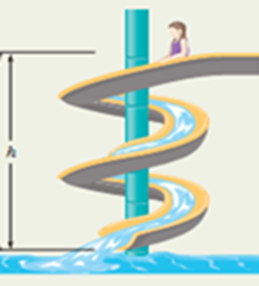
\includegraphics[scale=0.7]{../figs/VN10-2022-PH-TP029-1.png}
			\end{flushright}
		\end{minipage}
	}
	
	\hideall
	{	
			\begin{enumerate}[label=\alph*)]
			\item Tính vận tốc của bạn học sinh khi vừa chạm mặt nước.
			
			Chọn gốc thế năng tại mặt nước. Áp dụng bảo toàn cơ năng:
			$$W_1 = W_2 \Rightarrow 0 + mgz_1 = \dfrac{1}{2}mv_2^2 + 0 \Rightarrow v_2 = \xsi{10\sqrt 2}{m/s}.$$
			\item Ở độ cao nào bạn học sinh có động năng bằng 2 lần thế năng?
			
			Áp dụng bảo toàn cơ năng với $W_\text{đ 3} = 2 W_\text{t 3}$:
			$$W_1 = W_3 \Rightarrow W_1 = 2W_\text{t 3} + W_\text{t 3} = 3 mgz_3 \Rightarrow z_3 = \xsi{10/3}{m}.$$
		\end{enumerate}
	}
	\item \mkstar{3}
	
	
	{
			Một viên bi nhỏ khối lượng $\SI{200}{g}$ được ném thẳng đứng xuống dưới từ điểm O có độ cao $\SI{7}{m}$ so với mặt đất với tốc độ ban đầu $\SI{4}{m/s}$. Bỏ qua sức cản của không khí, lấy $g=\SI{10}{m/s^2}$. Giải bài toán bằng phương pháp năng lượng, chọn gốc thế năng tại mặt đất.
		\begin{enumerate}[label=\alph*)]
			\item Tìm độ cao của điểm M mà tại đó thế năng và động năng của viên bi bằng nhau.
			\item Tính tốc độ của viên bi ngay trước lúc chạm đất tại A.
		\end{enumerate}
	}
	
	\hideall
	{	
		\begin{enumerate}[label=\alph*)]
			\item Tìm độ cao của điểm M mà tại đó thế năng và động năng của viên bi bằng nhau.
			
			Khi $W_\text{đ M} = W_\text{t M}$ thì $\dfrac{1}{2}mv_\text{M}^2 = mgz_\text{M}$, áp dụng bảo toàn cơ năng tại O và M:
			$$W_\text{O} = W_\text{M} \Rightarrow \dfrac{1}{2}mv_\text{O}^2 + mgz_\text{O} = 2mgz_\text{M} \Rightarrow z_\text{M} = \SI{3.9}{m}.$$
			\item Tính tốc độ của viên bi ngay trước lúc chạm đất tại A.
			
			Áp dụng bảo toàn cơ năng tại O và A, với $z_\text{A} = 0$:
			$$W_\text{O} = W_\text{A} \Rightarrow \dfrac{1}{2}mv_\text{O}^2 + mgz_\text{O} = \dfrac{1}{2}mv_\text{A}^2 \Rightarrow v_\text{A} = \xsi{\sqrt{156}}{m/s}.$$
		\end{enumerate}
	}
	\item \mkstar{3}
	
	
	{
		Từ độ cao $\SI{10}{m}$ người ta thả rơi một vật khối lượng $\SI{2}{kg}$. Bỏ qua lực cản không khí, lấy $g=\SI{10}{m/s^2}$. Tính tốc độ của vật khi động năng của nó lớn hơn thế năng $\SI{60}{J}$.
	}
	
	\hideall
	{	
		Chọn gốc thế năng tại mặt đất. Gọi A, B lần lượt là vị trí thả vật và vị trí có động năng lớn hơn thế năng $\SI{60}{J}$. 
		
		Ta có $W_\text{đ B} = W_\text{t B} + 60 \Rightarrow W_\text{t B} = W_\text{đ B} - 60$.
		
		Áp dụng bảo toàn cơ năng tại A và B:
		$$W_\text{A} = W_\text{B} \Rightarrow 0 + mgz_\text{A} = W_\text{đ B} + (W_\text{đ B} - 60) = 2 W_\text{đ B} - 60 \Rightarrow v_\text{B} = \xsi{\sqrt{130}}{m/s}.$$
	}
	\item \mkstar{3}
	
	
	{
			Một vật có khối lượng $\SI{2}{kg}$ rơi tự do từ độ cao $h=\SI{100}{cm}$ xuống đất. Chọn gốc thế năng tại mặt đất, lấy $g=\SI{10}{m/s^2}$.
		\begin{enumerate}[label=\alph*)]
			\item Tính vận tốc cực đại trong quá trình chuyển động của vật.
			\item Khi động năng bằng 2 lần thế năng thì vật ở độ cao bao nhiêu?
		\end{enumerate}
	}
	
	\hideall
	{	
		\begin{enumerate}[label=\alph*)]
			\item Tính vận tốc cực đại trong quá trình chuyển động của vật.
			
			Vận tốc vật cực đại khi $z_2 = 0$, áp dụng bảo toàn cơ năng:
			$$W_1 = W_2 \Rightarrow 0 + mgz_1 = \dfrac{1}{2}mv_2^2 + 0 \Rightarrow v_2 = \xsi{2\sqrt5}{m/s}.$$
			\item Khi động năng bằng 2 lần thế năng thì vật ở độ cao bao nhiêu?
			
			Khi $W_\text{đ 3} = 2 W_\text{t 3}$ thì $W_3 = 3_\text{t 3}$. Áp dụng bảo toàn cơ năng:
			$$W_1 = W_3 \Rightarrow 0 + mgz_1 = 3 mgz_3 \Rightarrow z_3 = \xsi{1/3}{m}.$$
		\end{enumerate}
	}
	\item \mkstar{3}
	
	
	{
		Ở độ cao $\SI{10}{m}$ so với mặt đất, một vật khối lượng $m$ được ném thẳng đứng lên cao với vận tốc $\SI{36}{km/h}$. Chọn gốc thế năng tại mặt đất. Lấy $g=\SI{10}{m/s^2}$.
		\begin{enumerate}[label=\alph*)]
			\item Tính cơ năng của vật và độ cao cực đại mà vật đạt được.
			\item Tại vị trí vật có độ cao $\SI{4}{m}$, tính tỉ số giữa động năng và thế năng của vật.
		\end{enumerate}
	}
	
	\hideall
	{	
			\begin{enumerate}[label=\alph*)]
			\item Tính cơ năng của vật và độ cao cực đại mà vật đạt được.
			
			Cơ năng: $$W_1=\dfrac{1}{2}mv_1^2 + mgz_1 = \SI{15}{J}.$$
			
			Độ cao cực đại (tại $v_2 = 0$):
			$$W_1 = W_2 \Rightarrow \SI{15}{J} = mgz_2 \Rightarrow z_2 = \SI{15}{m}.$$
			
			\item Tại vị trí vật có độ cao $\SI{4}{m}$, tính tỉ số giữa động năng và thế năng của vật.
			
			Thế năng tại $z_3=\SI{4}{m}$:
			$$W_\text{t 3} = mgz_3 = \SI{4}{J}.$$
			
			Động năng tại đó:
			$$W_\text{đ 3} = W - W_\text{t 3} = \SI{11}{J}.$$
			
			Tỉ số động năng và thế năng là $11/4$.
		\end{enumerate}
	}
	\item \mkstar{3}
	
	
	{
		Một vật có khối lượng $\SI{400}{g}$ được ném thẳng đứng lên cao với vận tốc ban đầu $\SI{10}{m/s}$ ở độ cao $\SI{5}{m}$ so với mặt đất. Cho $g=\SI{10}{m/s^2}$. Bỏ qua lực cản không khí.
		\begin{enumerate}[label=\alph*)]
			\item Tính động năng, thế năng, cơ năng của vật lúc ném.
			\item Tính độ cao cực đại mà vật đạt được.
			\item Tính vận tốc của vật khi thế năng bằng 3 lần động năng.
		\end{enumerate}
		
	}
	
	\hideall
	{	
			\begin{enumerate}[label=\alph*)]
			\item Tính động năng, thế năng, cơ năng của vật lúc ném.
			
			Chọn gốc thế năng tại mặt đất.
			
			Động năng:
			$$W_\text{đ 1} = \dfrac{1}{2} mv_1^2  =\SI{20}{J}.$$
			
			Thế năng:
			$$W_\text{t 1} = mgz_1 = \SI{20}{J}.$$
			
			Cơ năng:
			$$W_1 = W_\text{đ 1} + W_\text{t 1} = \SI{40}{J}.$$
			
			\item Tính độ cao cực đại mà vật đạt được.
			
			Khi đó $v_2 = 0$. Áp dụng bảo toàn cơ năng:
			$$W_1 = W_2 \Rightarrow \SI{40}{J} = mgz_2 \Rightarrow z_2 = \SI{10}{m}.$$
			
			\item Tính vận tốc của vật khi thế năng bằng 3 lần động năng.
			
			Khi $W_\text{t 3} = 3 W_\text{đ 3}$ thì $W_3 = 4 W_\text{đ 3}$. Áp dụng bảo toàn cơ năng:
			$$W_1 = W_3 \Rightarrow \SI{40}{J} = 4 \cdot  \dfrac{1}{2}mv_3^2 \Rightarrow v_3 = \xsi{5\sqrt 2}{m/s}.$$
		\end{enumerate}
	}
	\item \mkstar{3}
	
	
	{
		Hòn đá khối lượng $m=\SI{0.5}{kg}$ buộc vào một dây dài $l=\SI{1.5}{m}$ quay trong mặt phẳng thẳng đứng. Biết lực căng của dây ở điểm thấp nhất của quỹ đạo có độ lớn là $T=\SI{45}{N}$.
		\begin{enumerate}[label=\alph*)]
			\item Tính vận tốc của hòn đá tại điểm thấp nhất.
			\item Tại vị trí mà vận tốc hòn đá có phương thẳng đứng hướng lên thì dây đứt. Hòn đá sẽ lên tới độ cao cực đại bao nhiêu tính từ nơi dây bắt đầu đứt?
		\end{enumerate}
	}
	
	\hideall
	{	
			\begin{enumerate}[label=\alph*)]
			\item Tính vận tốc của hòn đá tại điểm thấp nhất.
			
			Hợp lực của lực căng dây và trọng lực đóng vai trò lực hướng tâm. Chọn chiều dương là chiều hướng vào tâm, ta có:
			$$\vec T + \vec P = m\vec a_\text{ht} \Rightarrow T - P = m\dfrac{v^2}{l} \Rightarrow v \approx \SI{10.95}{m/s}.$$
			\item Tại vị trí mà vận tốc hòn đá có phương thẳng đứng hướng lên thì dây đứt. Hòn đá sẽ lên tới độ cao cực đại bao nhiêu tính từ nơi dây bắt đầu đứt?
			
			Chọn gốc thế năng tại điểm thấp nhất. Áp dụng định luật bảo toàn cơ năng cho vị trí thấp nhất và cao nhất:
			$$W_1 = W_2 \Rightarrow W_\text{đ 1} + W_\text{t 1} = W_\text{đ 2} + W_\text{t 2} \Rightarrow \dfrac{1}{2}mv_1^2 + 0 = 0 + mgz_2.$$
			$$\Rightarrow \dfrac{1}{2}mv_1^2 = mgz_2 \Rightarrow z_2 = \SI{6}{m}.$$
			
			So với vị trí dây bị đứt (có độ cao $h=l=\SI{1.5}{m}$ kể từ vị trí thấp nhất) thì hòn đá có thể lên đến độ cao cực đại là $$\SI{6}{m}-\SI{1.5}{m} = \SI{4.5}{m}.$$
		\end{enumerate}
	}
	\item \mkstar{3}
	
	
	{
		Một con lắc đơn gồm sợi dây nhẹ không dãn, chiều dài $\SI{50}{cm}$, một đầu cố định, đầu còn lại treo vật nặng có khối lượng $\SI{100}{g}$. Ban đầu vật nặng đứng yên ở vị trí cân bằng. Tại vị trí này, truyền cho vật nặng vận tốc $v_0=\SI{5}{m/s}$ theo phương ngang. Chọn gốc thế năng tại vị trí cân bằng và cho $g=\SI{10}{m/s^2}$.
		\begin{enumerate}[label=\alph*)]
			\item Tìm cơ năng của vật.
			\item Khi vật lên đến vị trí M có dây treo hợp với phương thẳng đứng góc $\alpha_\text M$, vật có thế năng bằng $1/4$ động năng. Hãy tính $\alpha_\text M$ và vận tốc của vật tại M.
		\end{enumerate}
	}
	
	\hideall
	{	
			\begin{enumerate}[label=\alph*)]
			\item Tìm cơ năng của vật.
			
			Cơ năng của vật bằng tổng động năng và thế năng:
			$$W_1 = \dfrac{1}{2}mv_1^2 + mgz_1 = \dfrac{1}{2}mv_1^2 + 0 = \SI{1.25}{J}.$$
			
			\item Khi vật lên đến vị trí M có dây treo hợp với phương thẳng đứng góc $\alpha_\text M$, vật có thế năng bằng $1/4$ động năng. Hãy tính $\alpha_\text M$ và vận tốc của vật tại M.
			
			Khi thế năng bằng $1/4$ động năng thì động năng gấp 4 lần thế năng, vậy cơ năng là
			
			$$W_2 = W_\text{đ 2} + W_\text{t 2} = 4 W_\text{t 2} + W_\text{t 2} = 5 W_\text{t 2} = W_1 \Rightarrow 5mgz_2 = \SI{1.25}{J} \Rightarrow z_2 = \SI{0.25}{m}.$$
			
			Mà góc $\alpha_\text M$ giữa phương thẳng đứng và phương dây treo được tính theo công thức: $\cos \alpha_\text M = \dfrac{l-z_2}{l} = \dfrac{1}{2}$, suy ra $\alpha_\text M = 60^\circ$.
			
			Vận tốc của vật tại M:
			$$W_\text{đ 2} = 4 W_\text{t 2} \Rightarrow \dfrac{1}{2}mv_2^2 = 4 mgz_2 \Rightarrow v_2 = \xsi{2\sqrt 5}{m/s}.$$
		\end{enumerate}
	}
	\item \mkstar{3}
	
	
	{
		Từ độ cao $\SI{25}{m}$ người ta ném thẳng đứng một vật nặng $\SI{50}{g}$ lên cao với vận tốc ban đầu bằng $\SI{20}{m/s}$. Bỏ qua sức cản không khí. Lấy $g=\SI{10}{m/s^2}$. Chọn gốc thế năng ở mặt đất.
		\begin{enumerate}[label=\alph*)]
			\item Tìm động năng, thế năng, cơ năng của vật ở vị trí ném.
			\item Khi thế năng của vật bằng nửa động năng, vật có độ cao và vận tốc bằng bao nhiêu?
			\item Tìm động năng của vật sau khi đi được $\SI{30}{m}$ kể từ lúc ném.
		\end{enumerate}
		
	}
	
	\hideall
	{	
			\begin{enumerate}[label=\alph*)]
			\item Tìm động năng, thế năng, cơ năng của vật ở vị trí ném.
			
			Động năng:
			$$W_\text{đ 1} = \dfrac{1}{2}mv_1^2  = \SI{10}{J}.$$
			
			Thế năng:
			$$W_\text{t 1} = mgz_1 = \SI{12.5}{J}.$$
			
			Cơ năng:
			$$W_1 = W_\text{đ 1} + W_\text{t 1} = \SI{22.5}{J}.$$
			
			\item Khi thế năng của vật bằng nửa động năng, vật có độ cao và vận tốc bằng bao nhiêu?
			
			Khi $W_\text{t 2} = \dfrac{1}{2} W_\text{đ 2}$ thì $W_\text{đ 2} = 2 W_\text{t 2}$. Áp dụng bảo toàn cơ năng:
			$$W_1 = W_2 \Rightarrow \SI{22.5}{J} = 3 W_\text{t 2} = 3 mgz_2 \Rightarrow z_2 = \SI{15}{m}.$$
			
			Khi đó $$W_\text{đ 2} = 2 W_\text{t 2} \Rightarrow \dfrac{1}{2}mv_2^2 = 2 mgz_2 \Rightarrow v_2 = \xsi{10\sqrt 6}{m/s}.$$
			
			\item Tìm động năng của vật sau khi đi được $\SI{30}{m}$ kể từ lúc ném.
			
			Độ cao cực đại mà vật đạt được:
			$$W_1 = W_3 \Rightarrow W_1 = 0 + mgz_3 \Rightarrow z_3 = \SI{45}{m}.$$
			
			Mà vật lúc đầu ở độ cao $\SI{25}{m}$, để đi được quãng đường $\SI{30}{m}$ thì vật sẽ lên đến độ cao cực đại rồi rơi xuống. Quãng đường từ $\SI{25}{m}$ đến $\SI{45}{m}$ là $\SI{20}{m}$. Vậy vật rơi xuống $\SI{10}{m}$ nữa là hoàn thành quãng đường $\SI{30}{m}$ theo yêu cầu. Nghĩa là khi đó vật ở vị trí cao $z_4 = \SI{45}{m} - \SI{10}{m} = \SI{35}{m}$.
			
			Áp dụng bảo toàn cơ năng:
			$$W_1 = W_4 \Rightarrow W_1 = W_\text{đ 4} + mgz_4 \Rightarrow \SI{22.5}{J} = W_\text{đ 4} + mgz_4 \Rightarrow W_\text{đ 4} = \SI{5}{J}.$$
		\end{enumerate}
	}
		\item \mkstar{3}
	
	
	{
		Thả rơi không vận tốc đầu một vật có khối lượng $m=\SI{200}{g}$ từ độ cao $h_0=\SI{5}{m}$ so với mặt đất. Lấy $g=\SI{10}{m/s^2}$ và bỏ qua mọi lực cản.
		\begin{enumerate}[label=\alph*)]
			\item Tính cơ năng của vật và tốc độ của vật khi vừa chạm đất.
			\item Tính thế năng và động năng của vật khi vật có động năng bằng 3 lần thế năng. Khi đó vật có tốc độ và độ cao bao nhiêu?
			\item Kể từ lúc thả, sau thời gian ngắn nhất bao lâu thì vật có thế năng bằng 3 lần động năng?
		\end{enumerate}
	}
	
	\hideall
	{	
			\begin{enumerate}[label=\alph*)]
			\item Tính cơ năng của vật và tốc độ của vật khi vừa chạm đất.
			
			Cơ năng:
			$$W_1 = mgh_0 + 0 = \SI{10}{J}.$$
			
			Khi vật chạm đất:
			$$W_1 = W_2 \Rightarrow \SI{10}{J} = \dfrac{1}{2} mv_2^2 + 0 \Rightarrow v_2 = \SI{10}{m/s}.$$
			
			\item Tính thế năng và động năng của vật khi vật có động năng bằng 3 lần thế năng. Khi đó vật có tốc độ và độ cao bao nhiêu?
			
			Ta có $W_\text{đ 3} = 3 W_\text{t 3}$ nên $W_3 = 4 W_\text{t 3} = \SI{10}{J}$, suy ra $W_\text{t 3} = \SI{2.5}{J}$, $z_3 = \SI{1.25}{m}$.
			
			Và $W_\text{đ 3} = \SI{7.5}{J}$, $v_3 = \xsi{5\sqrt 3}{m/s}$.
			
			\item Kể từ lúc thả, sau thời gian ngắn nhất bao lâu thì vật có thế năng bằng 3 lần động năng?
			
			Khi $W_\text{t 4} = 3W_\text{đ 4}$ thì $W_4 = \dfrac{4}{3} W_\text{t 4} = \dfrac{4}{3} mgz_4$, suy ra $z_4 = \SI{3.75}{m}$.
			
			Quãng đường vật rơi được: $s=h_0-z_4 = \SI{1.25}{m}$. Áp dụng công thức:
			$$s=\dfrac{1}{2}gt^2 \Rightarrow t = \SI{5}{s}.$$
		\end{enumerate}
	}
	\item \mkstar{3}
	
	
	{
		Một dây nhẹ dài $l=\SI{1}{m}$ đầu trên cố định, đầu dưới treo một vật nặng khối lượng $m$. Người ta kéo cho dây treo lệch một góc $\alpha = 60^\circ$ so với phương thẳng đứng rồi thả nhẹ cho vật chuyển động. Lấy $g=\SI{10}{m/s^2}$. Bỏ qua lực cản của không khí.
		\begin{enumerate}[label=\alph*)]
			\item Xác định vận tốc vật khi vật đi qua vị trí mà dây treo hợp với phương thẳng đứng một góc $\beta = 30^\circ$.
			\item Chứng minh rằng tại vị trí dây treo thẳng đứng vận tốc của vật có độ lớn cực đại, tìm giá trị cực đại đó.
		\end{enumerate}
	}
	
	\hideall
	{	
			\begin{enumerate}[label=\alph*)]
			\item Xác định vận tốc vật khi vật đi qua vị trí mà dây treo hợp với phương thẳng đứng một góc $\beta = 30^\circ$.
			
			Chọn gốc thế năng tại vị trí cân bằng của vật. Áp dụng định luật bảo toàn cơ năng:
			$$W_1 = W_2 \Rightarrow mgl(1-\cos \alpha) + 0 = \dfrac{1}{2} mv_2^2 + mgl (1-\cos \beta) \Rightarrow v_2 = \SI{2.7}{m/s}.$$
			
			\item Chứng minh rằng tại vị trí dây treo thẳng đứng vận tốc của vật có độ lớn cực đại, tìm giá trị cực đại đó.
			
			Tại vị trí dây treo thẳng đứng thì thế năng $z_3=0$, do đó động năng cực đại, dẫn đến vận tốc cực đại.
			
			Áp dụng bảo toàn cơ năng:
			$$W_1 = W_3 \Rightarrow mgl(1-\cos \alpha) = \dfrac{1}{2}mv_3^2 \Rightarrow v_3 = \xsi{\sqrt{10}}{m/s}.$$
		\end{enumerate}
	}
	\item \mkstar{3}
	
	
	{
		Vật nặng $\SI{2}{kg}$ trượt không vận tốc đầu từ đỉnh A của cung AB là $1/4$ cung tròn bán kính $R=\SI{2.4}{m}$. Sau đó tiếp tục trượt trên mặt ngang BC cách mặt đất độ cao $h=\SI{2}{m}$. Cho $g=\SI{10}{m/s^2}$. Bỏ qua ma sát, áp dụng dụng định luật bảo toàn cơ năng.
		\begin{enumerate}[label=\alph*)]
			\item Tính vận tốc của vật tại C.
			\item Đến C vật rơi ngang và rơi xuống đất. Tính vận tốc của vật khi vật chạm đất.
		\end{enumerate}
		\begin{center}
			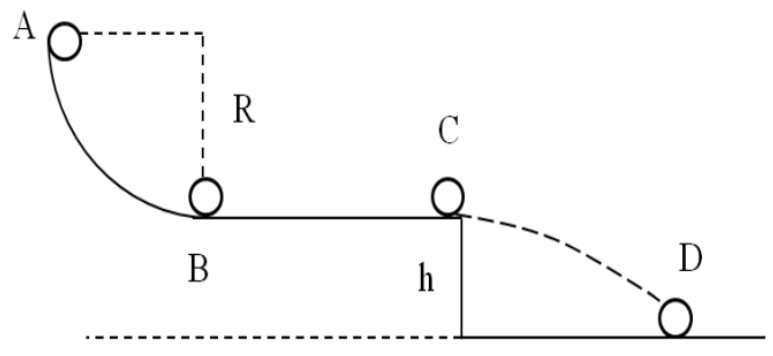
\includegraphics[scale=0.4]{../figs/VN10-2022-PH-TP029-4}
		\end{center}
	}
	
	\hideall
	{	
			\begin{enumerate}[label=\alph*)]
			\item Tính vận tốc của vật tại C.
			
			Chọn gốc thế năng tại mặt đất (tại D).
			
			Độ cao điểm A là $z_\text{A} = h + R = \SI{4.4}{m}$.
			
			Độ cao điểm C là $z_\text{C} = h = \SI{2}{m}$.
			
			Áp dụng bảo toàn cơ năng tại A và C:
			$$W_\text{A} = W_\text{C} \Rightarrow 0 + mgz_\text A = \dfrac{1}{2}mv_\text{C}^2 + mgz_\text{C} \Rightarrow v_\text{C} = \xsi{4\sqrt 3}{m/s}.$$
			
			\item Đến C vật rơi ngang và rơi xuống đất. Tính vận tốc của vật khi vật chạm đất.
			
			Áp dụng bảo toàn cơ năng tại C và D, với $z_\text{D} = 0$:
			$$W_\text{C} = W_\text{D} \Rightarrow \dfrac{1}{2}mv_\text{C}^2 + mgz_\text{C} = \dfrac{1}{2} mv_\text{D}^2 + 0 \Rightarrow v_\text{D} = \xsi{2\sqrt{22}}{m/s}.$$
		\end{enumerate}
	}
	\item \mkstar{3}
	
	
	{
		17h30 chiều 28-2, bé N.P.H. ở tầng 12A của tòa nhà 60B Nguyễn Huy Tưởng bò từ trong nhà, trèo ra lan can. Sau đó bé treo mình lơ lửng ở tầng 12A. Lúc này, một số người dân ở tòa bên cạnh phát hiện sự việc đã hô hoán. Một anh thanh niên đứng gần đó phát hiện sự việc nên trèo lên mái che của sảnh và đỡ được bé H. khi bé rơi xuống (\textit{Tuổi Trẻ Online}).
		
		Hành động dũng cảm của anh ấy giúp bảo toàn mạng sống cho cháu bé. Từ hiện tượng trên, học sinh hãy giải quyết bài toán vật lý sau:
		
		Vật $m_1=\SI{20}{kg}$ rơi tự do từ độ cao $h=\SI{40}{m}$ cách mặt đất. Khi đến đất, vật $m_1$ va chạm mềm với $m_2=\SI{60}{kg}$. Hãy tính phần năng lượng bị tiêu hao để làm nóng và làm biến dạng trong va chạm mềm giữa hai vật, biết rằng sau va chạm cả hai vật đều dừng chuyển động. Lấy $g=\SI{10}{m/s^2}$ và bỏ qua sức cản không khí.
	}
	
	\hideall
	{	
		Coi như vật $m_2$ nằm sát mặt đất, tổng cơ năng của hệ $m_1$ và $m_2$ lúc chưa xảy ra va chạm là:
		$$W = W_1 + W_2 = m_1gh = \SI{8000}{J}.$$
		
		Tổng cơ năng của hệ sau khi va chạm:
		$$W' = 0.$$
		
		Độ biến thiên cơ năng bằng phần năng lượng bị tiêu hao, do đó:
		$$\Delta W = \SI{8000}{J}.$$
	}
	\item \mkstar{3}
	
	
	{
		Một vật khối lượng $\SI{2}{kg}$ được ném thẳng đứng với vận tốc ban đầu $\SI{20}{m/s}$ xuống đất. Lấy $g=\SI{10}{m/s^2}$. Chọn gốc thế năng tại mặt đất. Bỏ qua lực cản của không khí trong quá trình vật chuyển động. Sau khi chạm đất, vật lún sâu $\SI{10}{cm}$ rồi dừng lại. Tính lực cản của đất.
	}
	
	\hideall
	{	
		Cơ năng của vật tại ví trí ném:
		$$W_1 = W_\text{đ 1} + W_\text{t 1} = \SI{400}{J}.$$
		
		Cơ năng của vật tại vị trí sâu $\SI{10}{cm}$ dưới đất:
		$$W_2 = 0 + mgz_2 = \SI{-2}{J}.$$
		
		Khi vật dừng lại thì toàn bộ cơ năng chuyển thành công của lực cản của đất:
		$$\Delta W = W_2 - W_1 = \SI{-402}{J}= A_\text{cản} = -F_\text{cản} \cdot \SI{0.1}{m} \Rightarrow F_\text{cản} = \SI{4020}{N}.$$
	}
	\item \mkstar{3}
	
	
	{
		Ném vật khối lượng $\SI{150}{g}$ thẳng đứng lên cao từ mặt đất với vận tốc $\SI{20}{m/s}$. Bỏ qua sức cản không khí. Cho $g=\SI{10}{m/s^2}$. Chọn gốc thế năng tại mặt đất.
		
		Nếu lực cản của không khí bằng $20\%$ trọng lượng của vật thì độ cao cực đại mà vật đạt được là bao nhiêu?
	}
	
	\hideall
	{	
			Cơ năng:
		$$W_1 = W_\text{đ 1} + 0 = \SI{30}{J}.$$
		
		Lực cản bằng $20\%$ trọng lượng của vật: $F_\text{cản} = \dfrac{20 mg}{100} = \SI{0.3}{N}$.
		
		Công của lực cản tác dụng lên vật từ khi vật ở mặt đất đến khi vật ở độ cao cực đại $h$:
		$$A_\text{cản} = -F_\text{cản} h.$$
		
		Độ biến thiên cơ năng bằng công của lực cản:
		$$\Delta W = W_2 - W_1 = mgh - W_1 = -F_\text{cản} h \Rightarrow h= \SI{16.67}{m}.$$
	}
		\item \mkstar{3}
	
	
	{
		Một viên bi nhỏ khối lượng $\SI{200}{g}$ được ném thẳng đứng xuống dưới từ điểm O có độ cao $\SI{7}{m}$ so với mặt đất với tốc độ ban đầu $\SI{4}{m/s}$. Bỏ qua sức cản của không khí, lấy $g=\SI{10}{m/s^2}$. Giải bài toán bằng phương pháp năng lượng, chọn gốc thế năng tại mặt đất. Đất mềm, viên bi lún thẳng xuống mặt đất thêm một đoạn $\SI{10}{cm}$. Tính lực cản trung bình của đất tác dụng lên viên bi.
	}
	
	\hideall
	{	
		Cơ năng của vật tại ví trí ném:
		$$W_1 = W_\text{đ 1} + W_\text{t 1} = \SI{15.6}{J}.$$
		
		Cơ năng của vật tại vị trí sâu $\SI{10}{cm}$ dưới đất:
		$$W_2 = 0 + mgz_2 = \SI{-0.2}{J}.$$
		
		Khi vật dừng lại thì toàn bộ cơ năng chuyển thành công của lực cản của đất:
		$$\Delta W = W_2 - W_1 = \SI{-15.8}{J}= A_\text{cản} = -F_\text{c} \cdot \SI{0.1}{m} \Rightarrow F_\text{cản} = \SI{158}{N}.$$
	}
	\item \mkstar{3}
	
	
	{
		Một vật có khối lượng $\SI{2}{kg}$ được thả rơi tự do từ độ cao $\SI{2.5}{m}$ so với mặt đất. Lấy $g=\SI{10}{m/s^2}$, bỏ qua mọi lực cản của không khí. Chọn gốc thế năng ở mặt đất.
		
		Khi rơi đến mặt đất, vật va chạm với mặt đất và nảy lên đến độ cao cực đại là $\SI{2}{m}$. Tìm phần cơ năng đã mất đi sau khi vật va chạm với mặt đất.
	}
	
	\hideall
	{	
		Cơ năng lúc thả vật (cơ năng trước khi vật va chạm với mặt đất):
		$$W_1 = mgz_1 = \SI{50}{J}.$$
		
		Cơ năng lúc vật nảy lên đến độ cao cực đại (cơ năng sau khi vật va chạm với mặt đất):
		$$W_2 = mgz_2 = \SI{40}{J}.$$
		
		Phần cơ năng đã mất đi: $$\Delta W = |W_2 - W_1| = \SI{10}{J}.$$
	}
	\item \mkstar{3}
	
	
	{
		\begin{minipage}[l]{0.7\textwidth}
			Vào tháng 1 năm 2020 tại trường THPT Lương Thế Vinh đã diễn ra cuộc thi đua xe thế năng dành cho học sinh khối 10 và khối 7. Cuộc thi đã diễn ra thành công, các học sinh thì hết sức hào hứng và có những trải nghiệm đáng nhớ.
			\begin{enumerate}[label=\alph*)]
				\item Trong cuộc đua, xe của các đội có thể được đặt thêm những thể tích chất lỏng khác nhau. Việc lựa chọn thể tích chất lỏng đặt vào xe có ảnh hưởng đến quãng đường xe đi được không? Tại sao?
				\item Dốc nghiêng được sử dụng để đua có độ dài $\SI{1.2}{m}$ và cao $\SI{40}{cm}$. Thân xe có khối lượng $\SI{1}{kg}$, lực ma sát xuất hiện trên mặt đất và dốc nghiêng không đổi và có độ lớn bằng $\SI{1.3}{N}$. Lấy $g=\SI{10}{m/s^2}$.
				
				Theo khảo sát, mối liên hệ giữa vận tốc của xe ở chân dốc và độ xa xe chạy được (kể từ chân dốc) được thống kê trong bảng phía dưới.
				\begin{center}
					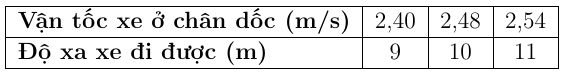
\includegraphics[scale=0.7]{../figs/VN10-2022-PH-TP029-7}
				\end{center}
				Dùng phương pháp năng lượng để giải quyết vấn đề sau đây: Bạn Thủy mong muốn xe của mình đạt được độ xa $\SI{10}{m}$ thì bạn cần phải đổ vào xe một lượng nước bao nhiêu? Biết rằng 1 lít nước có khối lượng 1 kg.
			\end{enumerate}
		\end{minipage}
		\begin{minipage}[r]{0.25\textwidth}
			\begin{flushright}
				
\includegraphics[width=0.7\linewidth]{../figs/VN10-2022-PH-TP029-2}
				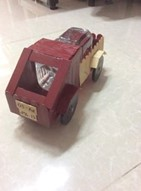
\includegraphics[width=0.7\linewidth]{../figs/VN10-2022-PH-TP029-6}
			\end{flushright}			
		\end{minipage}
	}
	
	\hideall
	{	
			\begin{enumerate}[label=\alph*)]
			\item Việc lựa chọn thể tích chất lỏng đặt vào xe (thay đổi khối lượng xe) không ảnh hưởng đến quãng đường xe đi được. Xét trên quãng đường xe đi được từ vị trí chân dốc đến khi xe dừng lại, theo định lý biến thiên cơ năng, khối lượng của vật ở cả 2 vế của định lý triệt tiêu nhau:
			$$0 - \dfrac{1}{2}mv_1^2 = - \mu mg s$$
			
			\item Để xe đi được độ xa $s=\SI{10}{m}$ thì theo bảng thống kê, vận tốc xe ở chân dốc phải là $v_1 = \SI{2.48}{m/s}$.
			
			Chọn gốc thế năng tại chân dốc. Áp dụng biến thiên cơ năng cho xe lúc ở chân dốc và lúc ở độ xa $\SI{10}{m}$:
			$$\Delta W = W_2 - W_1 = A_\text{ms} \Rightarrow (0+0) - (\dfrac{1}{2}mv_1^2 + 0) = -F_\text{ms} s \Rightarrow m = \SI{4.23}{kg}.$$
			
			Mà thân xe nặng $\SI{1}{kg}$ nên thể tích nước cần đổ vào xe là $\SI{3.23}{kg}$, tương ứng $\SI{3.23}{l}$ nước.
		\end{enumerate}
	}
	\item \mkstar{3}
	
	
	{
		Ném một vật thẳng đứng lên trên với vận tốc $\SI{5}{m/s}$ từ độ cao $\SI{1.5}{m}$ so với mặt đất. Bỏ qua mọi lực cản, cho $g=\SI{10}{m/s^2}$.
		\begin{enumerate}[label=\alph*)]
			\item Tính độ cao cực đại mà vật đạt được và quãng đường mà vật đi được từ khi đạt độ cao cực đại đến khi vật có thế năng bằng 4 lần động năng.
			\item Khi vật đến mặt đất tại điểm D, do đất mềm nên vật lún vào đất $\SI{20}{cm}$. Tính công của lực cản trung bình của đất tác dụng lên vật. Biết khối lượng vật bằng $\SI{400}{g}$.
		\end{enumerate}
	}
	
	\hideall
	{	
			\begin{enumerate}[label=\alph*)]
			\item Tính độ cao cực đại mà vật đạt được và quãng đường mà vật đi được từ khi đạt độ cao cực đại đến khi vật có thế năng bằng 4 lần động năng.
			
			Chọn gốc thế năng tại mặt đất. Áp dụng bảo toàn cơ năng tại vị trí ném và vị trí độ cao cực đại:
			$$W_\text{A} = W_\text{B} \Rightarrow \dfrac{1}{2}mv_\text{A}^2 + mgz_\text{A} = 0 + mgz_\text{B} \Rightarrow z_\text{B} = \SI{2.75}{m}.$$
			
			Khi vật có thế năng bằng 4 lần động năng $W_\text{t C} = 4 W_\text{đ C}$ thì $W_\text{C} = \dfrac{W_\text{t C}}{4} + W_\text{C} = \dfrac{5 W_\text{t C}}{4}$. Áp dụng bảo toàn cơ năng:
			$$W_\text{A} = W_\text{C} \Rightarrow \dfrac{1}{2}mv_\text{A}^2 + mgz_\text{A} = \dfrac{5 mgz_\text{C}}{4}  \Rightarrow z_\text{C} = \SI{2.2}{m}.$$
			
			Vậy quãng đường vật đi được từ khi đạt độ caoc cực đại đến khi vật có thế năng bằng 4 lần động năng là $s=z_\text{B} - z_\text{C} = \SI{0.55}{m}$.
			
			\item Khi vật đến mặt đất tại điểm D, do đất mềm nên vật lún vào đất $\SI{20}{cm}$. Tính công của lực cản trung bình của đất tác dụng lên vật. Biết khối lượng vật bằng $\SI{400}{g}$.
			
			Cơ năng tại điểm D có $z_\text{D} = \SI{-0.2}{m}$: $W_\text{D} = mgz_\text{D} = \SI{-0.8}{J}$
			
			Độ biến thiên cơ năng bằng công của lực cản:
			$$A_\text{cản} = \Delta W = W_\text{D} - W_\text{A} = \SI{-11.8}{J}.$$
		\end{enumerate}
	}
	\item \mkstar{3}
	
	
	{
		Một vật có khối lượng $\SI{3}{kg}$ được thả rơi không vận tốc đầu từ độ cao $\SI{4}{m}$ so với mặt đất. Lấy $g=\SI{9.8}{m/s^2}$. Biết ngay trước khi chạm đất vận tốc của vật là $\SI{6}{m/s}$. Hãy tính lực cản trung bình của không khí tác dụng lên vật.
	}
	
	\hideall
	{	
		Chọn gốc thế năng tại mặt đất. Cơ năng vật lúc mới thả vật:
		$$W_1 = 0 + mgz_1 = \SI{117.6}{J}.$$
		
		Cơ năng vật ngay trước khi vật chạm đất:
		$$W_2 = \dfrac{1}{2}mv_2^2 + 0 = \SI{54}{J}.$$
		
		Độ biến thiên cơ năng bằng công của lực cản (với $s=\SI{4}{m}$):
		$$W_2 - W_1 = -F_\text{cản} s \Rightarrow F_\text{cản} = \SI{15.9}{N}.$$
	}
	\item \mkstar{3}
	
	
	{
		Từ tầng 10 của tòa nhà cao tầng cách mặt đất $\SI{35}{m}$, một vật nặng $\SI{200}{g}$ được ném theo hướng xuống với vận tốc $\SI{20}{m/s}$. Chọn mốc thế năng tại mặt đất, bỏ qua mọi ma sát và lực cản của không khí, lấy $g=\SI{10}{m/s^2}$. Khi rơi xuống đất, do đất mềm và lún thì người ta thấy vật lún sâu vào đất một đoạn. Biết lực cản trung bình của đất là $\SI{440}{N}$. Tìm độ sâu vật lún vào đất.
	}
	
	\hideall
	{	
		Cơ năng lúc ném vật:
		$$W_1 = \dfrac{1}{2}mv_1^2 + mgz_1 = \SI{110}{J}.$$
		
		Cơ năng vật lúc vật ở độ sâu $d$ trong đất:
		$$W_2 = -mgd.$$
		
		Độ biến thiên cơ năng bằng công của lực cản:
		$$W_2 - W_1 = -F_\text{c} d \Rightarrow -mgd - W_1 = -F_\text{c} d \Rightarrow d = \SI{0.25}{m}.$$
		
		Vậy độ sâu vật lún vào đất là $d=\SI{0.25}{m}$.
	}
		\item \mkstar{3}
	
	
	{
		Một vật trượt không vận tốc đầu từ đỉnh mặt phẳng nghiêng cao $\SI{1.25}{m}$. Cho gia tốc rơi tự do $g=\SI{10}{m/s^2}$.
		\begin{enumerate}[label=\alph*)]
			\item Vật trượt không ma sát trên mặt phẳng nghiêng. Hãy tính vận tốc của vật tại chân mặt phẳng nghiêng.
			\item Khi đến chân mặt phẳng nghiêng, vật tiếp tục trượt trên mặt phẳng nằm ngang nối liền với mặt nghiêng. Thời gian chuyển động của vật trên mặt phẳng ngang là $\SI{5}{s}$. Tính hệ số ma sát giữa vật và mặt phẳng nằm ngang.
		\end{enumerate}
	}
	
	\hideall
	{	
		\begin{enumerate}[label=\alph*)]
			\item Vật trượt không ma sát trên mặt phẳng nghiêng. Hãy tính vận tốc của vật tại chân mặt phẳng nghiêng.
			
			Chọn gốc thế năng tại mặt đất. Bảo toàn cơ năng tại đỉnh dốc và chân dốc:
			$$W_1 = W_2 \Rightarrow 0 + mgz_1 = \dfrac{1}{2}mv_2^2 + 0 \Rightarrow v_2 = \SI{5}{m/s}.$$
			
			\item Khi đến chân mặt phẳng nghiêng, vật tiếp tục trượt trên mặt phẳng nằm ngang nối liền với mặt nghiêng. Thời gian chuyển động của vật trên mặt phẳng ngang là $\SI{5}{s}$. Tính hệ số ma sát giữa vật và mặt phẳng nằm ngang.
			
			Gia tốc của vật trên mặt nghiêng:
			$$v_3 = 0 = at + v_2 \Rightarrow a = \SI{-1}{m/s^2}.$$
			
			Quãng đường vật trượt trên mặt ngang:
			$$s=\dfrac{1}{2}at^2 + v_2 t = \SI{12.5}{m}.$$
			
			Độ biến thiên cơ năng bằng công của lực ma sát:
			$$W_3 - W_2 = -\mu mg s \Rightarrow 0 - \dfrac{1}{2}mv_2^2 = -\mu mg s \Rightarrow \mu = \SI{0.1}{}.$$	
			
		\end{enumerate}
	}
	\item \mkstar{3}
	
	
	{
			\begin{minipage}[l]{0.7\textwidth}
			
			Một vật lăn lên dốc từ A với vận tốc $\SI{10}{m/s}$, vật dừng lại ở B rồi lăn xuống dốc theo đường cũ. Tốc độ vật khi xuống chân dốc ở A là $\SI{6}{m/s}$. Cho $g=\SI{10}{m/s^2}$ và hệ số ma sát $\mu = \SI{0.1}{}$. Tìm AC.
			
		\end{minipage}
		\begin{minipage}[r]{0.25\textwidth}
			\hspace*{0.9cm}
			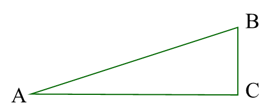
\includegraphics[scale=0.5]{../figs/VN10-2022-PH-TP029-5}
		\end{minipage}
	}
	
	\hideall
	{	
			Độ biến thiên cơ năng của vật trong suốt quá trình chuyển động:
		$$\Delta W = \dfrac{1}{2} m (v_2^2 - v_1^2)=-32m.$$
		
		Công của lực ma sát trong quá trình vật chuyển động lên (với $l=\text{AB}$):
		
		$$A_\text{ms 1} = -\mu mg \cos \alpha l.$$
		
		Công của lực ma sát trong quá trình vật chuyển động xuống:
		$$A_\text{ms 2} = -\mu mg \cos \alpha l.$$
		
		Công của lực ma sát trong suốt quá trình:
		$$A_\text{ms} = - 2\mu mg \cos \alpha l.$$
		
		Mà độ biến thiên cơ năng bằng công của lực ma sát, suy ra
		$$\Delta W = -32m = - 2\mu mg \cos \alpha l \Rightarrow 32 =\mu g \cos \alpha l.$$
		
		Lại có $\cos \alpha = \dfrac{\text{AC}}{l}$ nên:
		$$32 =\mu g \dfrac{\text{AC}}{l} l = \mu g \text{AC} \Rightarrow \text{AC} = \SI{32}{m}.$$
	}
	\item \mkstar{3}
	
	
	{
			Một lò xo nhẹ có độ cứng $k=\SI{50}{N/m}$, một đầu cố định, đầu còn lại gắn vào vật khối lượng $m=\SI{100}{g}$. Vật có thể chuyển động không ma sát trên mặt sàn nằm ngang song song với trục lò xo. Từ vị trí cân bằng người ta kéo vật ra khỏi vị trí cân bằng một đoạn $x_1$ và thả nhẹ cho vật chuyển động. Khi vật đến vị trí cân bằng, vật có tốc độ $\xsi{20\sqrt 5}{cm/s}$. Tìm $x_1$ và độ lớn lực đàn hồi tại vị trí lò xo dãn $x_1$.
	}
	
	\hideall
	{	
			Cơ năng của hệ tại vị trí thả vật:
		$$W_1 = \dfrac{1}{2}kx_1^2 +0 = \dfrac{1}{2}kx_1^2.$$
		
		Cơ năng của hệ tại vị trí vật trở lại vị trí cân bằng (với $v=\xsi{0.2\sqrt5}{m/s}$):
		$$W_2 = 0 + \dfrac{1}{2}mv^2 = \dfrac{1}{2}mv^2.$$
		
		Bảo toàn cơ năng:
		$$W_1 = W_2 \Rightarrow \dfrac{1}{2}kx_1^2 = \dfrac{1}{2}mv^2 \Rightarrow x_1 = \SI{2}{cm}.$$
		
		Lực đàn hồi tại vị trí lò xo dãn $\SI{0.02}{m}$:
		$$F_\text{đh} = -kx_1 = \SI{-1}{N}.$$
	}
	\item \mkstar{3}
	
	
	{
		Một hệ gồm lò xo có độ cứng $\SI{100}{N/m}$ gắn với vật nhỏ có khối lượng $\SI{500}{g}$. Hệ được đặt trên mặt bàn nằm ngang, đầu còn lại của lò xo được gắn vào điểm cố định, kéo vật để lò xo dãn ra $\SI{4}{cm}$ rồi thả nhẹ không vận tốc đầu. Bỏ qua lực ma sát giữa vật và mặt bàn, chọn gốc thế năng tại vị trí lò xo không biến dạng. Tìm thế năng đàn hồi của lò xo tại vị trí buông vật và tính công của lực đàn hồi đã thực hiện khi vật di chuyển từ vị trí được thả đến vị trí lò xo dãn $\SI{2}{cm}$.
	}
	
	\hideall
	{	
			Thế năng đàn hồi của lò xo tại vị trí buông vật (với $\Delta l_1 = \SI{0.04}{m}$):
		
		$$W_\text{t 1} = \dfrac{1}{2}k(\Delta l_1)^2 = \SI{0.08}{J}.$$
		
		Công của lực đàn hồi bằng độ giảm thế năng (với $\Delta l_2 = \SI{0.02}{m}$):
		
		$$A=W_\text{t 1} - W_\text{t 2} =\dfrac{1}{2}k(\Delta l_1^2 - \Delta l_2^2) =\SI{0.06}{J}.$$
	}
	\item \mkstar{3}
	
	
	{
		Khối gỗ $M=\SI{4}{kg}$ nằm trên mặt phẳng nằm ngang trơn nhẵn, nối với tường bằng lò xo có độ cứng $k=\SI{100}{N/m}$, trục lò xo song song với mặt phẳng nằm ngang. Viên đạn $m=\SI{10}{g}$ bay theo phương ngang với vận tốc $v_0$ song song với trục của lò xo đến đập vào và dính trong gỗ. Sau va chạm, lò xo bị nén một đoạn tối đa là $\Delta l = \SI{30}{cm}$. Tìm $v_0$.	
	}
	
	\hideall
	{	
			Áp dụng định luật bảo toàn động lượng trước và sau va chạm cho hệ viên đạn - khối gỗ:
		$$\vec p_1 = \vec p_2 \Rightarrow mv_0 + 0 = (M+m)V \Rightarrow V = \dfrac{v_0}{401}.$$
		
		Cơ năng của hệ ngay sau khi va chạm:
		$$W_1 = W_\text{đ 1} + 0 = \dfrac{1}{2} (M+m)V^2.$$
		
		Cơ năng của hệ khi lò xo bị nén một đoạn $\Delta l = \SI{30}{cm}$:
		$$W_2 = 0 + W_\text{t 2} = \dfrac{1}{2} k (\Delta l)^2.$$
		
		Vì bỏ qua ma sát, áp dụng bảo toàn cơ năng:
		$$W_1 = W_2 \Rightarrow \dfrac{1}{2} (M+m)V^2 = \dfrac{1}{2} k (\Delta l)^2 \Rightarrow \dfrac{1}{2} (M+m) \cdot \left(\dfrac{v_0}{401}\right)^2 =  \dfrac{1}{2} k (\Delta l)^2 \Rightarrow v_0 \approx \SI{600.75}{m/s}.$$
	}
	\item \mkstar{3}
	
	
	{
		Một lò xo có chiều dài tự nhiên $l_0=\SI{25}{cm}$ đặt trên mặt phẳng nằm ngang. Một đầu lò xo cố định, đầu kia gắn với vật nhỏ $m_1$. Ban đầu giữ vật $m_1$ tại vị trí mà lò xo bị nén một đoạn $\SI{8}{cm}$, đặt vật nhỏ $m_2$ (với $m_2=3m_1$) trên mặt phẳng nằm ngang sát với vật $m_1$. Buông nhẹ để hai vật bắt đầu chuyển động theo phương của trục lò xo. Bỏ qua mọi ma sát. Tính chiều dài cực đại của lò xo.
	}
	
	\hideall
	{	
			Cơ năng ban đầu của hệ:
		$$W_1 = \dfrac{1}{2}kx^2.$$
		
		Hệ bao gồm vật $m_1$ dính với $m_2$ chuyển động cùng nhau từ lúc buông nhẹ đến khi hệ ở vị trí lò xo không biến dạng. Tại vị trí lò xo không biến dạng thì vật $m_2$ tách khỏi $m_1$, khi đó hệ chỉ còn vật $m_2$ và ta không xét đến vật $m_1$ nữa.
		
		Cơ năng của hệ tại vị trí cân bằng ngay trước khi $m_2$ tách ra:
		$$W_2 = \dfrac{1}{2} (m_1+m_2)v^2 = \dfrac{1}{2} (4m_1) v^2.$$
		
		Cơ năng của hệ tại vị trí cân bằng ngay sau khi $m_2$ tách ra:
		$$W_2' = \dfrac{1}{2}m_1v^2.$$
		
		Vậy $W_2'= \dfrac{W_2}{4} = \dfrac{W_1}{4}$, suy ra:
		$$\dfrac{1}{2}k x'^2 = \dfrac{1}{4} \cdot \dfrac{1}{2}kx^2 \Rightarrow x'^2 = \dfrac{1}{4}x^2 \Rightarrow x'=\SI{4}{cm}.$$
		
		Vậy chiều dài cực đại của lò xo cần tìm là $l_\text{max} = \SI{25}{cm} + \SI{4}{cm} = \SI{29}{cm}$.
	}
	
\end{enumerate}